\documentclass[draft]{lecturenotes}

\usepackage{mlbasemath}
\usepackage{mlprobabilita}
\usepackage{pgfplots}       % per i grafici
\pgfplotsset{compat=1.5}    % consigliata compatibilita'
                            % con la versione 1.5

\newtheorem{exmp}{Esempio}

\begin{document}

\title{Calcolo delle probabilit\`a}

\maketitle

\newpage

\tableofcontents
\newpage

\chapter{Calcolo combinatorio}

\section{Principio fondamentale del calcolo combinatorio}

\begin{theorem}
Consideriamo $n$ esperimenti (un meta-esperimento di $n$ esperimenti, come il lancio di due dadi = 2 esperimenti). Supponiamo che il primo esperimento abbia $m_1$ esiti possibili. Qualunque sia l'esito del primo esperimento il secondo esperimento ha sempre $m_2$ esiti possibili. Qualunque sia il risultato (coppia di esiti) dei primi due esperimenti, il terzo esperimento ha $m_3$ esiti possibili, e cos\`i via. Gli esiti possibili di ogni esperimento sono sempre gli stessi, qualunque sia il risultato degli esperimenti precedenti.

Allora il meta-esperimento ha $ m_1 \times m_2 \times m_3 \times \dots \times m_n $ stringhe possibili nella forma $( a_1, a_2, a_3, \dots a_n)$, dove $a_1$ \`e l'esito dell'esperimento $i$-esimo $\forall \ i \in [1, n]$.
\end{theorem}

Dati due insiemi finiti $A$ e $B$, voglio determinare la cardinalit\`a delle funzioni da $A$ a $B$.
\begin{gather*}
\sharp \left\{ f: A \to B \right\} \\
\abs{\left\{ f: A \to B \right\}}
\end{gather*}
$\abs{A} = n$, $\abs{B} = m$. Considero un elemento di $A$, $a_1$, ho $m$ modi di decidere la sua immagine in $B$. Per ogni altro elemento di $A$, ho sempre $m$ modi di decidere la sua immagine in $B$. Ho quindi $n$ fattori tutti pari ad $m$, per cui il risultato \`e $m^n$.

Altro esempio: il numero delle sigle di cinque caratteri ottenute usando le 26 lettere dell'alfabeto inglese. $26^5$

Se la sigla fosse composta da cinque caratteri senza ripetizioni? $26 \times 25 \times 24 \times 23 \times 22$.

\section{Permutazioni ed anagrammi}

Le permutazioni sono i possibili ordinamenti di un insieme di $n$ oggetti distinti. I due insiemi $ \left\{ A, C, Z, X \right\}$ e $ \left\{ A, Z, X, C \right\} $ sono lo stesso insieme. ACZX e AZXC \textit{non} sono la stessa permutazione.

Con l'insieme $\{A,C,Z,X\}$ posso scegliere il primo elemento di una permutazione in 4 modi possibili, il secondo in 3, il terzo in 2, il quarto in 1. Quindi ho $4!$ permutazioni.

Le permutazioni di un insieme di $n$ oggetti distinti sono $n!$

\textit{Gli aggettivi in matematica sono colpi d'accetta.}

Ma ora voglio gli anagrammi di MATTEO. Non sono lettere distinte. Considero quindi un alfabeto esteso in cui ho $T_1$ e $T_2$. In questo alfabeto esteso, il numero di anagrammi possibili sono 6! Da questa lista devo cancellare i numeri sotto le T. Quante ripetizioni ho per ogni anagramma? Tante quanto il numero di modi in cui posso combinare le lettere ripetute, in questo caso $2!$

Ciascun anagramma \`e ripetuto $2!$ volte. Il numero di anagrammi \`e:
\[
\frac{6!}{2!}
\]
VITTORIO, tre lettere si ripetono due volte. La parola ha 8! anagrammi, se numero le lettere ripetute. Considero un anagramma, ORIOVITT. Posso numerare ciascuna lettera ripetuta in 2! modi, quindi ho $2! \times 2! \times 2!$ modi per mettere gli indici alle lettere.
\[
\frac{8!}{2! \times 2! \times 2!}
\]
ZOZZO, $5!$ anagrammi numerando le lettere. Z ripetuta 3 volte, O ripetuta 2 volte.
\[
\frac{5!}{3! \times 2!}
\]
Consideriamo una famiglia di $n$ oggetti con ripetizioni: vi sono $r$ tipi di oggetti, il primo tipo si presenta $n_1$ volte, il secondo tipo $n_2$ volte e cos\`i via. Notiamo: $ n_1 + n_2 + \dots + n_r = n$. I possibili ordinamenti di questa famiglia sono:
\[
\frac{ n! }{ n_1! \times n_2! \times \cdots \times n_r!}
\]

\section{Sottoinsiemi di una certa dimensione}

Ho un insieme di $n$ oggetti distinti. In quanti modi posso scegliere $r$ oggetti da questo insieme, indipendentemente dall'ordine in cui li scelgo? Coincide con la domanda: quanti sono i possibili sottoinsiemi di cardinalit\`a $r$ di un insieme di cardinalit\`a $n$? Necessariamente $r \leq n$, altrimenti la risposta sarebbe 0.

Se l'ordine contasse, avrei $n \times (n-1) \times (n-2) \times \cdots \times (n-r+1)$ modi per scegliere gli $r$ oggetti.

Ogni gruppo di $r$ oggetti pu\`o essere disposto in $r!$ modi differenti. Quindi se dimentico l'ordine avr\`o $r!$ ``copie'' ci ciascun gruppo di $r$ oggetti. Un insieme di $r$ elementi ha $r!$ permutazioni (ordinate) $\implies$ per ogni $r$-upla non ordinata ho $r!$ $r$-uple ordinate.

Rispondendo alla domanda:
\[
\frac{(n) \ (n-1) \ \ldots \ (n - r + 1)}{r!} =
\frac{ n! }{ r! \ (n-r)! } = 
\binom{n}{r}
\]
Ricordiamo i coefficienti binomiali. Con $0 \le r \le n$:
\[
\binom{n}{k} = \frac{n!}{k! \ (n-k)!} = 
\frac{n \ (n - 1) \ (n - 2) \ldots (n - k + 1)}{k!}
\]
Se $r \geq n \implies \binom{n}{r} = 0$. Propriet\`a dei coefficienti binomiali:
\[
\binom{n}{r} = \binom{n}{n-r}
\]
Da cui $\binom{n}{n} = \binom{n}{0} = 1$. \`E una ``bigezione''. Se ho un insieme $X$ di cardinalit\`a $\abs{X} = n$, ed un suo sottoinsieme $A$ con il suo complementementare $B = X \setminus A$, il numero di modi in cui posso scegliere $A$ sono uguali al numero di modi in cui posso scegliere $B$.
\begin{align*}
\left\{A \subset X : \abs{A} = r\right\} \\
\left\{B \subset X : \abs{B} = n - r\right\}
\end{align*}
Con $1 \leq r \leq n$:
\[
\binom{n}{r} = \binom{n-1}{r-1} + \binom{n-1}{r}
\]
Ciao Salvo. Con $X = V \cup W$ e $X \setminus V = W$, $\abs{X} = \abs{V} + \abs{W}$.

I coefficienti binomiali si leggono anche ``$n$ scelgo $k$''. I coefficienti binomiali servono con i binomi:
\begin{multline*}
(a+b)^n = 
a^n 
+ \binom{n}{1} \, b \, a^{n-1} 
+ \binom{n}{2} \, b^2 \, a^{n-2} 
+ \ldots 
+ \binom{n}{n-2} \, b^{n-2} \, a^2
+ \binom{n}{n-1} \, b^{n-1} \, a
+ b^n
\end{multline*}
\[
(x+y)^n = \sum_{k=0}^{n} \binom{n}{k} \, x^k \, y^{n-k}
\]
Un esempio lievemente pi\`u complementicato: devo scegliere un rappresentante e due segretari da un gruppo di ottanta persone. Ho ottanta modi per scegliere il rappresentante. Mi restano 79 persone da cui devo scegliere una coppia non ordinata. Per il principio fondamentale del calcolo combinatorio:
\[
80 \times \binom{79}{2} = \frac{80 \times 79 \times 78}{2!}
\]
Ho $r$ tipi di oggetti, ciascun tipo ha $n_i$ oggetti distinti, con $i \in [1,r]$. In quanti modi posso \textit{raggruppare} gli oggetti per tipo? Ho $r!$ modi per disporre i tipi di oggetti, gli oggetti del tipo $i$ possono essere disposti in $n_i!$ modi. Per il principio fondamentale del calcolo combinatorio:
\[
r! \times n_1! \times n_2! \times \cdots \times n_r! = 
r! \prod_{k = 1}^{r} n_r!
\]
Remember: $0! = 1$.
\[
\sum_{k=0}^{n} \binom{n}{k} = \sum_{k=0}^{n} \binom{n}{k} \, 1^k \, 1^{n-k} = (1 + 1)^n = 2^n
\]
O anche mi basta sapere che $\binom{n}{k}$ \`e il numero di sottoinsiemi di $k$ elementi di un insieme di $n$ elementi. Tutti i sottoinsiemi sono l'insieme delle parti, che ha cardinalit\`a $2^n$.

$X$ insieme con cardinalit\`a $\abs{X} = n$. $\parts(X) = \left \{ Y : Y \subset X \right\}$. Un sottoinsieme $Y \subset X$ pu\`o o non pu\`o contenere ciascun elemento di $X$. Quanti sottoinsiemi $Y$ posso costruire?
\[
\overbrace{2 \times 2 \times 2 \times \dots \times 2}^{n} = 2^n
\]
Un modo pi\`u complesso per dimostrarlo:
\begin{align*}
\parts(X) = \left \{Y :  Y \subset X \right\} = \bigcup_{k=0}^{n} \left \{ Y \subset X : \abs{Y} = k \right\} \\
\abs{\parts(X)} = \sum_{k=0}^{n} \abs{\left\{ Y \subset X : \abs{Y} = k\right\}}  = \sum_{k = 0}^{n} \binom{n}{k}
\end{align*}

\section{Coefficienti multinomiali}

Ho 10 persone. Devo assegnare 5 persone al compito 1, 2 al compito 2, 3 al compito 3. In quanti modi posso farlo?
\[
\binom{10}{5} \binom{5}{2} \binom{3}{3} = 
\frac{10!}{5! \ 5!} \ \frac{5!}{2! \ 3!} \ \frac{3!}{3! \ 0!} =
\frac{10!}{5! \ 3! \ 2!}
\]
Ho un insieme di $n$ oggetti distinti e $k$ categorie in cui inserirli. Devo inserire $n_1$ elementi nella categoria 1, $n_2$ elementi nella categoria 2, \dots $n_k$ elementi da inserire nella categoria $k$, senza che nessuno resti fuori, ossia $\sum_{i = 1}^{k} n_i = n$, con $n_i \in \naturals \forall i \in [1, k]$. In quanti modi lo posso fare?

\begin{align*}
\binom{n}{n_1} \binom{n - n_1}{n_2} \binom{n - (n_1 + n_2)}{n_3}\dots \binom{n - \left( \sum_{i = 1}^{k-1} n_i \right)}{n_k} = \\
\binom{n}{n_1} \binom{n - n_1}{n_2} \binom{n - (n_1 + n_2)}{n_3}\dots \binom{n_k}{n_k} = \\
\frac{n!}{n_1! \left( n - n_1\right)!} \ 
\frac{(n - n_1)!}{n_1! \left( n - n_1 - n_2\right)!} \ 
\frac{(n - n_1 - n_2)!}{n_1! \left( n - n_1 - n_2 - n_3\right)!} \ 
\dots \\
\frac{(n - n_1 - n_2 \dots - n_{k-2})!}{n_1! \left( n - n_1 - n_2 \dots - n_{k-2} - n_{k-1} \right)!} \ 
\frac{(n - n_1 - n_2 \dots - n_{k-1})!}{n_1! \ 0!} = \\
\frac{n!}{\prod_{i=1}^{k}n_k!} =
\binom{n}{n_1, n_2, \dots, n_k}
\end{align*}
Detto anche coefficiente multinomiale. Ricordiamo che $\sum_{i = 1}^{k} n_i = n$. I coefficienti binomiali sono un caso particolare dei coefficienti multinomiali. Sapendo che $n = n_1 + n_2$:
\[
\binom{n}{n_1, n_2} = \binom{n}{n_1, n - n_1} = \frac{n!}{n_1! (n - n_1)!} = \binom{n}{n_1}
\]
Devo dividere $n$ persone ($n$ pari) in 2 gruppi. Dopo generalizziamo a $m$ gruppi (spero) con $n$ multiplo di $m$. Se i gruppi fossero distinguibili avrei:
\[
\binom{n}{\frac{n}{2}, \frac{n}{2}}
\] 
modi per formare i gruppi. Ma non essendo distinguibili i gruppi avr\`o:
\[
\frac{\binom{n}{\frac{n}{2}, \frac{n}{2}}}{2} = \frac{n!}{2 \ \frac{n}{2}! \ \frac{n}{2}!} = \frac{n \ (n - 1) \dots (\frac{n}{2}+1)}{2 \frac{n}{2}!} = \frac{(n-1)(n-2) \dots (\frac{n}{2} + 1)}{(\frac{n}{2}-1)!} = \binom{n-1}{\frac{n}{2}-1}
\] 
\section{Teorema multinomiale}
Con $n_i \ge 0$ interi:
\[
\left( x_1 + \dots + x_r \right)^n = 
\sum_{n_1 + \dots + n_r = n} \binom{n}{n_1, \dots, n_r} \cdot x_1^{n_1} \cdots x_r^{n_r}
\]
Wikipedia lo scrive come:
\[
\left( \sum_{i=1}^r x_i \right)^n=\sum_{k_1+\ldots+k_r=n}{n!\cdot \prod_{i=1}^r \frac{x_i^{k_i}}{k_i!}}
\]





















\newpage

\chapter{Calcolo della Probabilit\`a}


\section{Spazio di probabilit\`a}

Consideriamo un esperimento con pi\`u esiti possibili. Vogliamo modellizzarlo con uno ``spazio di probabilit\`a''.

\begin{defn}[Spazio campionario]
Chiamiamo l'insieme dei possibili esiti dell'esperimento $S$, ``spazio campionario''.
\end{defn}

\begin{defn}[Evento]
Matematicamente, un \emph{evento} \`e un sottoinsieme dello spazio campionario. Ad esempio, con lo spazio campionario dei risultati di un dado $\{ 1, 2, 3, 4, 5, 6\}$ un evento potrebbe essere ``esce un numero pari'', che corrisponde all'insieme di esiti $\{2, 4, 6\}$.

Un evento elementare \`e un sottoinsieme dello spazio campionario consistente di un singolo elemento (o esito): $\{ s \}, s \in S$.
\end{defn}

\begin{defn}[Spazio e funzione di probabilit\`a]
Lo spazio di probabilit\`a che modellizza l'esperimento \`e una coppia $(S,P)$ dove $S$ \`e lo spazio campionario e $P$ \`e una funzione reale, detta ``funzione di probabilit\`a'' definita su $\parts(S)$ t.c. valgono i seguenti assiomi:
\begin{description}
    \item[P1\label{itm:P1}] $0 \le \prob{E} \le 1 \forall  E \subset S$, la funzione di probabilit\`a associa un numero fra 0 ed 1 ad ogni \emph{evento}, non ad ogni esito. La probabilit\`a di un evento \`e un numero fra 0 ed 1.
    \item[P2\label{itm:P2}] $\prob{S} = 1$. $S$ \`e l'``evento certo'', la cui probabilit\`a \`e 1.
    \item[P3\label{itm:P3}] Assioma di numerabile additivit\`a: se $E_1, E_2, \dots$ \`e una successione di eventi ($E_1 \subset S \forall  i$), a 2 a 2 disgiunti (o incompatibili) ($E_i \cap E_j = \emptyset$ se $i \neq j$), allora:
    \[
    \prob{\bigcup_{i=1}^{\infty} E_i} = \sum_{i=1}^{\infty} \prob{E_i}
    \]
    Vuol dire che, considerando eventi incompatibili, la probabilit\`a dell'unione \`e la somma delle probabilit\`a. 
\end{description}
\end{defn}

L'insieme delle parti di $S$ \`e la ``famiglia degli eventi'', la funzione $P: \parts(S) \to [0,1]$. La funzione $P$ \`e definita sull'insieme delle parti di $S$.

L'intero insieme $S$ rappresenta l'evento certo. L'insieme vuoto $\emptyset$ \`e l'evento impossibile.

Se $E, F$ sono eventi con $E \cap F = \emptyset \implies E$ ed $F$ sono detti ``incompatibili'': il realizzarsi di un evento implica che l'altro non si \`e realizzato. 

$\prob{\emptyset} = 0$ non \`e un'assioma. Prendo infiniti insiemi a due a due disgiunti $E_1, E_2, \dots, E_n$ dove $E_i = \emptyset$, e quindi $\bigcup_{n=1}^{\infty} E_n = \emptyset$. Per l'assioma di numerabile additivit\`a:
\[
\prob{\emptyset} = \sum_{n=1}^{\infty} \prob{\emptyset} \implies \prob{\emptyset} = 0
\]
L'unico elemento che sommato infinite volte a s\'e stesso d\`a sempre s\'e stesso \`e lo 0.

\begin{prop}[Additivit\`a finita \label{additivita_finita}]
$P$ soddisfa l'additivit\`a finita. Considerata una famiglia finita $E_1, E_2, \dots, E_k$ di eventi a due a due disgiunti, vale che $\prob{\bigcup_{n=1}^k E_n} = \sum_{n=1}^k \prob{E_n}$.
\end{prop}
\begin{proof}
Consideriamo la successione di eventi $F_1, F_2, F_3, \dots$ cos\`i definita:
\[
F_n =
\begin{cases}
E_n \text{ se } 1 \le n \le k \\
\emptyset \text{ se } n > k
\end{cases}
\]
Ho quindi una successione infinita di eventi a due a due disgiunti. Posso applicare l'assioma di numerabilit\`a additiva:
\[
\prob{\bigcup_{n = 1}^{\infty} F_n} = \sum_{n = 1}^{\infty} \prob{F_n}
\]
Ma $\bigcup_{n = 1}^{\infty} F_n = \bigcup_{n = 1}^{k} E_n$, quindi:
\[
\prob{\bigcup_{n = 1}^{\infty} F_n} =
\prob{\bigcup_{n = 1}^{k} E_n} =
\sum_{n = 1}^{\infty} \prob{F_n}
\]
Inoltre $\prob{F_n}$ \`e definita come:
\[
\prob{F_n} =
\begin{cases}
\prob{E_n} \text{ se } 1 \le n \le k \\
\prob{\emptyset} \text{ se } n >k
\end{cases}
\]
Quindi:
\[
\sum_{n = 1}^{\infty} \prob{F_n} =
\sum_{n = 1}^{k} \prob{E_n}
\]
Per transitivit\`a ho dimostrato la tesi.
\[
\prob{\bigcup_{n=1}^k E_n} = \sum_{n=1}^k \prob{E_n}
\]
\end{proof}

L'additivit\`a richiede la disgiunzione.

\begin{prop}[Probabilit\`a dell'evento complementare]
Dato un evento $E$, l'evento complementare $E^{\compl} = S \setminus E$ ha probabilit\`a:
\[
\prob{E^{\compl}} = 1 - \prob{E}
\]
\end{prop}
\begin{proof}
Applico la proposizione \ref{additivita_finita} con $k = 2$, dato che i due insiemi sono disgiunti.
\[
\prob{E \cup E^{\compl}} = \prob{E} + \prob{E^{\compl}}
\]
Ma poich\'e $E + E^{\compl} = S$:
\[
\prob{E \cup E^{\compl}} = \prob{E} + \prob{E^{\compl}} = P(S) = 1 \implies
\prob{E^{\compl}} = 1 - \prob{E}
\]
\end{proof}

\begin{prop}[Monotonia della compatibilit\`a]
Se $E$ e $F$ sono eventi compatibili ($E \subset F$), allora $\prob{E} \le \prob{F}$. Sapendo che $F = E \cup (F \setminus E)$:
\[
\prob{F} = \prob{E \cup (F \setminus E)} = \prob{E} + \prob{F \setminus E} \ge \prob{E}
\]
\end{prop}

Dati due eventi $A, B \subset S$ tali che $A \cap B = \emptyset \implies \prob{A \cup B} = \prob{A} + \prob{B}$. Ma nel caso generale?

\begin{prop}
Dati due eventi $A$, $B \subset S$, vale che $\prob{A \cup B} = \prob{A} + \prob{B} - \prob{A \cap B}$. La cardinalit\`a, come la misura della probabilit\`a, \`e additiva: $\abs{A \cup B} = \abs{A} + \abs{B} - \abs{A \cap B}$.
\end{prop}
\begin{proof}
Dati due eventi congiunti $A, B$, chiamiamo $I = A \setminus B$, $II = A \cap B$, $III = B \setminus A$. $A \cup B = I \cup II \cup III$. Essendo i tre insiemi disgiunti, posso applicare l'additivit\`a finita.
\[
\prob{A \cup B} = \prob{I} + \prob{II} + \prob{III}
\]
Sempre per l'additivit\`a finita: $\prob{A} = \prob{I} + \prob{II}$ e $\prob{B} = \prob{II} + \prob{III}$, e $\prob{A \cap B} = \prob{II}$. Riscrivo quindi il membro destro della proposizione come:
\begin{align*}
\prob{A} + \prob{B} - \prob{A \cap B} = \\
\prob{I} + \prob{II} + \prob{II} + \prob{III} - \prob{II} = \\
\prob{I} + \prob{II} + \prob{III} = \\
\prob{A \cup B}
\end{align*}
E ho dimostrato la tesi.
\end{proof}

\section{Spazi campionar\^i  a esiti equiprobabili}

Quale \`e lo spazio di probabilit\`a $(S,P)$ che descrive il lancio di un dado?
\[
S = \{ 1, 2, 3, 4, 5, 6 \}
\]
Ma qual \`e la funzione di probabilit\`a $P : \parts(S) \to [0,1]$? Non ho motivi per ritenere che una faccia esca pi\`u spesso rispetto alle altre. Per simmetria, le probabilit\`a degli eventi elementari $\prob{\{1\}} = \prob{\{2\}} = \dots = \prob{\{6\}}$ sono tutte uguali.
\begin{align*}
\prob{S} &= 1 = \prob{\{1,2,\dots, 6\}} = \tag{per la propriet\`a \ref{itm:P2}} \\
&= \underbrace{\prob{\{1\}}}_{x} + \prob{\{2\}} + \dots + \prob{\{6\}} = \tag{per additivit\`a finita} \\
&= 6 \cdot x \implies \\
& x = \frac{\prob{S}}{6} = \frac{1}{6} = \prob{\{k\}}
\end{align*}
% Riprendendo la propriet\`a \ref{itm:P2}, $\prob{S} = 1 = \prob{\{1,2,\dots, 6\}}$. Ma per l'additivit\`a finita, $\prob{S} = P(\{1\}) + P(\{2\}) + \dots + P(\{6\})$. Sono tutti numeri uguali, per cui $P(S) = 6 \ x$ con $x = P(\{1\})$. Quindi:
% \[
% x = \frac{P(S)}{6} = \frac{1}{6} = P(\{k\})
% \]

Sappiamo quindi la probabilit\`a di un evento elementare. Ma qual \`e $\prob{E}$ con $E \subseteq S$?
\[
\prob{E} = \prob{\bigcup_{k \in E} \{k\}}
\]
\`E una famiglia finita di insiemi a due a due disgiunti, quindi per l'additivit\`a finita:
\[
\prob{E} = \sum_{k \in E} \prob{\{k\}} = \frac{\abs{E}}{6} = \frac{\abs{E}}{\abs{S}}
\]
La probabilit\`a di un evento \`e data dal numero degli esiti favorevoli diviso il numero degli esiti equiprobabili, ma solo se gli esiti \emph{sono} equiprobabili.

\begin{defn}[Spazio di probabilit\`a con esiti equiprobabili]
Uno spazio di probabilit\`a $(P,S)$ \`e detto con esiti equiprobabili se $\prob{\{s\}} = \prob{\{s'\}} \forall s, s' \in S$.
\end{defn}
\begin{prop}
Sia $S$ finito e $(S,P)$ con esiti equiprobabili, allora:
\[
\prob{E} = \frac{\abs{E}}{\abs{S}} \qquad \forall  E \subseteq S
\]
\end{prop}
\begin{proof}
Dato un evento $E$, posso scrivere:
\[
E = \bigcup_{s \in E} \{ s \}
\]
ossia, $E$ \`e un'unione finita di eventi a due a due disgiunti. Posso quindi applicare l'additivit\`a finita:
\[
\prob{E} = \sum_{s \in E} \prob{\{s\}}
\]
Consideriamo il caso in cui $E = S$:
\[
\prob{S} = \sum_{s \in S} \underbrace{\prob{\{ s \}}}_{x} = x \cdot \abs{S}
\]
poich\'e $\prob{\{s\}} = x$ non dipende da $s \in S$. Quindi $x = \frac{1}{\abs{S}}$, con $x = \prob{\{s\}} \forall  s \in S$. Sostituisco nell'equazione precedente:
\[
P(E) = \sum_{s \in E} \frac{1}{|S|} = \frac{|E|}{|S|}
\]
\end{proof}

\begin{prop}
Sia $\abs{S} = + \infty$ e $S$ numerabile, non esiste uno spazio di probabilit\`a con esiti equiprobabili. 
\end{prop}
\begin{proof}
Supponiamo per assurdo che esista $(S,P)$ con esiti equiprobabili. So che $P(S) = 1$, e che:
\[
S = \bigcup_{s \in S} \{s\}
\]
Ho un'unione infinita numerabile di eventi a due a due disgiunti. Applico l'additivit\`a numerabile:
\[
P(S) = \sum_{s \in S} \underbrace{P \left( \{ s \} \right)}_{x} = 1
\]
Non esiste un numero $x$ che sommato infinite volte da 1, o qualunque altro numero finito.
\end{proof}

\begin{esercizio}
Lancio due volte un dado.
\begin{itemize}
    \item Modellizare l'esperimento con uno spazio di probabilit\`a;
    \item Calcolare la probabilit\`a che escano gli stessi numeri.
\end{itemize}
Lo spazio campionario \`e $S = \{ (a,b) : a,b \in \{ 1 \dots 6 \} \}$, con $a$ faccia del primo lancio e $b$ faccia del secondo lancio. In un singolo lancio ogni faccia \`e equivalente ad ogni altra faccia. La simmetria vale ancora se faccio due lanci. Quindi:
\[
\forall  E \subseteq S \qquad P(E) = \frac{|E|}{|S|} = \frac{|E|}{36}
\]

Prendiamo l'evento $E = $ ``le due facce sono uguali''. $E = \{ (1,1), (2,2) \dots (6,6) \}$.
\[
P(E) = \frac{6}{36} = \frac{1}{6}
\]
\end{esercizio}

\begin{esercizio}
Ho un'urna contenente 8 palline blu, 5 gialle e 3 nere. Estraggo tre palline senza rimpiazzo. Qual \`e la probabilit\'a di estrarre tre palline blu?

Non posso definire lo spazio campionario basandomi sul colore: estrarre una pallina blu e una gialla, ad esempio, non \`e un esito equiprobabile. Posso distinguere le palline dello stesso colore numerandole. In questo caso estrarre una pallina rispetto ad un'altra \`e equiprobabile.
\end{esercizio}

\section{Principio di inclusione-esclusione}

So che, dati gli eventi $A$ e $B$ non necessariamente disgiunti, la probabilit\`a della loro unione \`e $P(A \cup B) = P(A) + P(B) - P(A \cap B)$. Se volessi generalizzare a $n$ eventi?

\begin{prop}
Dati $n$ eventi $E_1, E_2 \dots E_n$, vale che:
\begin{align*}
P(E_1 \cup E_2 \cup \dots \cup E_n) = \\
P(E_1) + P(E_2) + \dots + P(E_n) \\
- \sum_{1 \le i_1 < i_2 \le n} P(E_{i_1} \cap E_{i_2}) \\
+ \sum_{1 \le i_1 < i_2 < i_3 \le n} P(E_{i_1} \cap E_{i_2} \cap E_{i_3}) \\
\dots \\
+ (-1)^{n+1} P(E_1 \cap E_2 \cap \dots \cap E_n)
\end{align*}
In maniera pi\`u compatta:
\begin{equation}
P(E_1 \cup E_2 \cup \dots \cup E_n) =
\sum_{r = 1}^{n} (-1)^{r+1} 
\left(
\sum_{1 \le i_1 < i_2 < \dots < i_r \le n} P(E_{i_1} \cap E_{i_2} \cap \dots \cap E_{i_r})
\right)
\end{equation}
\end{prop}
\begin{exmp}
Prendiamo tre eventi $E, F, G$ (in seguito scriveremo $EF$ per intendere $E \cap F$) e vediamo la probabilit\`a di $P(E \cup F \cup G)$.
\begin{align*}
P(E \cup F \cup G) = \\
(-1)^{1+1} \ (P(E) + P(F) + P(G)) \\
+ (-1)^{2+1} \ (P(E \cap F) + P(E \cap G) + P(F \cap G)) \\
+ (-1)^{3+1} \ (P(E \cap F \cap G)) = \\
P(E) + P(F) + P(G) - P(E \cap F) - P(E \cap G) - P(F \cap G) + P(E \cap F \cap G)
\end{align*}
\end{exmp}
\begin{proof}
Limitiamo la dimostrazione a $S$ numerabile. Se lo spazio campionario \`e numerabile, vale la proposizione \ref{numerabile}.

Dato $s \in S$ e dato $E \subseteq S$ indichiamo con il simbolo $\mathbf{1}(s \in E)$ (funzione caratteristica associata alla propriet\`a ``$s \in E$'') la funzione:
\[
\mathbf{1}(s \in E) =
\begin{cases}
1 \text{ se } s \in E \\
0 \text{ se } s \notin E 
\end{cases}
\]
Quindi la proposizione \ref{numerabile} equivale a scrivere:
\[
P(E) = \sum_{s \in E} P(\{s\}) = \sum_{s \in S} \mathbf{1}(s \in E) P(\{s\})
\]
Posso riscrivere il membro sinistro della proposizione come:
\[
P(E_1 \cup E_2 \cup \dots \cup E_n) = 
\sum_{a \in S} \mathbf{1}(a \in E_1 \cup \dots \cup E_n) P(\{a\})
\]
Posso riscrivere il membro destro della proposizione come:
\[
\sum_{r = 1}^{n} (-1)^{r+1} 
\left(
\sum_{1 \le i_1 < i_2 < \dots < i_r \le n} 
\overbrace{
P(E_{i_1} \cap E_{i_2} \cap \dots \cap E_{i_r})
}^{ \sum_{a \in S} \mathbf{1}(a \in E_1 \cap \dots \cap E_n) P(\{a\}) }
\right) 
\]
Il risultato di una serie a termini non costanti dipende dall'ordine di somma. Ma queste serie sono assolutamente convergenti, quindi posso scambiare l'ordine di somma. Quindi:
\[
\sum_{a \in S} P(\{a\}) \left[ \sum_{r = 1}^n (-1)^{r+1} \sum_{1 \le i_1 < \dots < i_r \le n} \mathbf{1}(a \in E_{i_1} \cap E_{i_2} \cap \dots \cap E_{i_r}) \right]
\]
Per dimostrare il principio di inclusione-esclusione basta dimostrare che, $\forall  a \in S$:
\[
\sum_{r = 1}^n (-1)^{r+1} \sum_{1 \le i_1 < \dots < i_r \le n} \mathbf{1}(a \in E_{i_1} \cap E_{i_2} \cap \dots \cap E_{i_r}) = \mathbf{1}(a \in E_1 \cup \dots \cup E_n)
\]
Il membro destro sar\`a sempre o 0 o 1, il membro sinistro sar\`a una somma di 1, 0 e $-1$. Distinguiamo due casi:
\begin{enumerate}
    \item $a \notin E_1 \cup \dots \cup E_n$, allora il membro destro vale 0. Ma quindi $a$ non pu\`o appartenere all'intersezione di eventi, se non appartiene alla loro unione. Quindi anche il membro sinistro \`e 0 (o una somma di 0).
    \item $a \in E_1 \cup \dots \cup E_n$, allora il membro destro vale 1. Sia $m$ il numero degli eventi di tipo $E_i$ a cui $a$ appartiene (ossia per cui $a \in E_i$). Per semplicit\`a, ma senza perdita di generalit\`a, supponiamo che $a$ appartenga ai primi $m$ elementi. Abbiamo quindi che $\mathbf{1}(a \in E_{i_1} \cap \dots \cap E_{i_r}) = 1 \Leftrightarrow i_1, i_2, \dots i_r \le m$.

    Quindi la somma dei valori della funzione caratteristica per valori fino a $m$ \`e uguale al numero di possibili tuple di numeri distinti ordinati in senso crescente compresi fra 1 e $m$.
    \[
    \sum_{1 \le i_1 < \dots < i_r \le n} \mathbf{1}(a \in E_{i_1} \cap E_{i_2} \cap \dots \cap E_{i_r}) = \left| \{(i_1,i_2, \dots i_r) : 1 \le i_1 < i_2 < \dots < i_r \le m\} \right|
    \]
    Altro non \`e che $\binom{m}{r}$. C'\`e una bigezione fra il numero di insiemi non ordinati e il numero di $n$-uple ordinate in senso crescente.

    La parte sinistra dell'equazione vale quindi:
    \[
    \sum_{r = 1}^{n} (-1)^{r+1} \binom{m}{r}
    \]
    Dobbiamo dimostrare che \`e uguale ad 1. Se $r > m$ il coefficiente binomiale vale 0. La somma si pu\`o semplificare ancora e diventare quindi:
    \[
    \sum_{r = 1}^{m} (-1)^{r+1} \binom{m}{r} =
    \sum_{r = 0}^{m} (-1)^{r+1} \binom{m}{r} + 1 =
    - \sum_{r = 0}^{m} (-1)^{r} \binom{m}{r} + 1
    \]
    Posso riscrivere tutto con il teorema del binomio applicato a $(1 - 1)^m$:
    \[
    \sum_{r = 0}^{m} \binom{m}{r} 1^{m-r} (-1)^r + 1 = (1-1)^m + 1 = 0 + 1 = 1
    \]
\end{enumerate}
\end{proof}
\begin{prop}\label{numerabile}
Sia $S$ numerabile (finito o infinito), Allora $\forall  E \subset S$ vale:
\[
P(E) = \sum_{s \in E} P(\{s\})
\]
\end{prop}
\begin{proof}
Se $S$ \`e numerabile $\implies E$ \`e numerabile (perch\'e la cardinalit\`a di un insieme \`e maggiore della cardinalit\`a di un suo sottoinsieme proprio). Posso scrivere $E$ come:
\[
E = \bigcup_{s \in E} \{ s \}
\]
ossia, un'unione numerabile di eventi a due a due disgiunti. Vale quindi che:
\[
P(E) = \sum_{s \in E} P(\{s\})
\]
\end{proof}

\begin{prop}
Supponiamo di avere una famiglia di eventi $E_1, E_2, \dots E_n$ vale che:
\[
P(E_1 \cup E_2 \cup \dots \cup E_n) \le P(E_1) + P(E_2) + \dots + P(E_n)
\]
Inoltre, data una successione di eventi $E_1, E_2, \dots E_n \dots$ vale che:
\[
P \left( \bigcup_{n = 1}^{\infty} E_n \right) \le \sum_{n = 1}^{\infty} P(E_n)
\]
\end{prop}
\begin{proof}
Dimostriamo solo la prima parte. Per $n = 2$ vale che $P(E_1 \cup E_2) = P(E_1) + P(E_2) - P(E_1 \cap E_2) \le P(E_1) + P(E_2)$.

Concludiamo per induzione. Se vale per $n$, vale per $n + 1$. Pensiamo $ P(E_1 \cup E_2 \cup \dots \cup E_n \cup E_{n+1}) $ come $P( A \cup E_{n+1})$ con $A = E_1 \cup E_2 \cup \dots \cup E_n$.
\[
P(E_1 \cup E_2 \cup \dots \cup E_n \cup E_{n+1}) \le P(E_1 \cup \dots \cup E_n) + P(E_{n+1}) \le P(E_1) + \dots + P(E_n) + P(E_{n+1})
\]
\end{proof}

\begin{exmp}
Abbiamo cinque coppie, ciascuna formata da un uomo e una donna. Vogliamo sapere qual \`e la probabilit\`a di prendere $G_i = F_i$ balla con $M_i$.
\[
E^{\compl} = G_1 \cup G_2 \cup G_3 \cup G_4 \cup G_5
\]
\[
P(E^c) = P(G_1 \cup G_2 \cup G_3 \cup G_4 \cup G_5) = \sum_{r = 1}^{5} (-1)^{r +1} \sum_{1 \le i_1 < i_2 \dots i_r \le 5} P( G_{i_1} \cap G_{i_2} \dots G_{i_r})
\]
$P(G_i)$ non dipende da $i$, per simmetria.
\[
P(G_1) = \frac{4!}{5!} = \frac{1}{5}
\]
Sappiamo che \`e vero $\forall i = 1 \dots 5$. In generale:
\[
P( G_{i_1} \cap \dots \cap G_{i_r}) = \frac{(5 - r)!}{5!}
\]
\[
P(E) = 1 - \sum_{r = 1}^{5} (-1)^{r+1} \frac{1}{r!} = 
\sum_{k = 0}^{5} \frac{(-1)^k}{k!}
\]
Quindi:
\[
P(E) = 1 - \frac{1}{1!} + \frac{1}{2!} - \frac{1}{3!} + \frac{1}{4!} - \frac{1}{5!} = 
\frac{3 \cdot 4 \cdot 5 - 4 \cdot 5 + 5 - 1}{5!}
\]
In generale:
\[
\sum_{k = 0}^{N} \frac{(-1)^k}{k!}
\]
Per $N$ all'infinito, questo \`e lo sviluppo in serie di $e^{-1}$
\end{exmp}
\section{Interpretazione frequentistica della probabilit\`a}

Ripeto un esperimento $N$ volte. Chiamo $K(E, N)$ il numero di volte in cui $E$ si \`e verificato tra gli $N$ esperimenti. Quindi il rapporto $\frac{K(E, N)}{N}$ \`e la frequenza relativa con cui $E$ si \`e verificato negli $N$ esperimenti.

Per $N$ grande la frequenza relativa \`e circa la probabilit\`a di $E$.
\[
\frac{K(E,N)}{N} \approx P(E)
\]
Di norma aggiungo informazioni per rendere gli esiti simmetrici.

La modellizzazione si basa sul buon senso. La funzione di probabilit\`a in caso di esiti non equiprobabili si costruisce statisticamente.

Su 1000 lanci, il mio dado truccato mi d\`a:

\begin{tabular}{cc}
1 & 405 \\
2 & 200 \\
3 & 001 \\
4 & 103 \\
5 & 050 \\
6 & 241
\end{tabular}

Modellizzo quindi il mio dado con una funzione di probabilit\`a $P : \parts(S) \to [0,1]$ viene definita su $S = \{ 1 \dots 6 \}$ come:
\begin{align*}
P(\{1\}) &= \frac{405}{1000} \\
P(\{2\}) &= \frac{200}{1000} \\
\dots & \\
P(\{6\}) &= \frac{241}{1000}
\end{align*}

Abbiamo la probabilit\`a degli eventi elementari. Se sappiamo la probabilit\`a degli eventi elementari, sappiamo tutto. Infatti per $S$ numerabile (finito o infinito):
\[
P(E) = \sum_{s \in E} P(\{s\})
\]
\begin{prop}
Se $S$ \`e numerabile, allora per ogni funzione $p : S \to [0,1]$ tale che $\sum_{s \in S} p(s) = 1 \exists ! P$ funzione di probabilit\`a con $P(\{s\}) = p(s) \forall  s \in S$.
\end{prop}

\section{Probabilit\`a condizionata}

Probabilit\`a condizionata all'informazione. Abbiamo un'informazione parziale sul risultato dell'esperimento.

\begin{defn}[Probabilit\`a condizionata]
Dati due eventi $E$ e $F$ con $P(F) > 0$ si definisce la probabilit\`a di $E$ condizionata dall'evento $F$ come:
\[
P(E|F) = \frac{P(E \cap F)}{P(F)} 
\]
\end{defn}

\begin{oss}
Se $S$ ha esiti equiprobabili e se $\abs{S} < + \infty$, allora:
\[
P(E|F) = \frac{\abs{E \cap F}}{\abs{F}}
\]
\end{oss}

\begin{proof}
Siccome lo spazio ha esiti equiprobabili, scriviamo la formula come cardinalit\`a di insiemi:
\[
P(E|F) = \frac{P(E \cap F)}{P(F)} = \frac{\frac{\abs{E \cap F}}{\abs{S}}}{\frac{\abs{F}}{\abs{S}}} = \frac{\abs{E \cap F}}{\abs{F}}
\]
Se moltiplico per $N$ numero di esperimenti, ho che $P(F)\ N$ \`e il numero di volte in cui si \`e verificato $P(F)$ negli $N$ esperimenti, e $P(E \cap F) \ N$ \`e il numero di volte in cui si \`e verificato sia $E$ che $F$.
\end{proof}

Lancio due dadi. $F =$ ``la somma dei due dadi \`e 7''. Qual \`e la probabilit\`a $E =$ ``il secondo lancio ha dato 3''?

% gioco delle tre carte, RR RN NN

\subsection{Legge del prodotto (o legge delle probabilit\`a composte)}
\begin{theorem}[Legge del prodotto]
Siano $E_1, E_2, \ldots, E_n$ eventi con $P(E_1 \cap \ldots \cap E_{n-1}) > 0$, allora:
\[
P(E_1 \cap \ldots \cap E_{n}) = P(E_1) \ P(E_2 | E_1) \ P(E_3 | E_1 \cap E_2) \ \ldots \ P(E_n | E_1 \cap E_2 \cap \ldots \cap E_{n-1})
\]
$P(E|F)$ si legge ``probabilit\`a di E condizionato F''.
\end{theorem}

\begin{exmp}
Ho un'urna contenente 5 palline blu, 3 rosse e 6 gialle. Estraggo 3 palline senza rimpiazzo e voglio sapere la probabilit\`a che siano tutte gialle. Definisco, immaginando di estrarre le palline una dopo l'altra, l'evento $E_i =$ ``la pallina $i$-esima \`e gialla'', per $i = 1, 2, 3$. $P(E_1 \cap E_2 \cap E_3)$ \`e la probabilit\`a che tutte le palline siano gialle. Per la legge delle probabilit\`a composte quindi:
\[
P(E_1 \cap E_2 \cap E_3) = 
P(E_1) \ P(E_2 | E_1) \ P(E_3 | E_1 \cap E_2)
\]
Al momento di estrarre la prima pallina so che la probabilit\`a di estrarre una pallina gialla \`e $P(E_1) = \frac{6}{14}$
\end{exmp}

La probabilit\`a condizionata ha senso quando l'evento condizionante ha cardinalit\`a positiva.

\begin{oss}
$P(E_1 \cap \ldots \cap E_{n_1}) > 0 \implies \forall r = 1 \dots n - 1 , \, P(E_1 \cap E_2 \cap \ldots \cap E_r) > 0$.
\end{oss}

Se $F \subset E$ e $P(F) > 0$ allora $P(E) > 0$

\begin{proof}
Il membro destro \`e:
\[
P(E_1) \cdot \frac{P(E_1 \cap E_2)}{P(E_1)} \cdot \frac{P(E_1 \cap E_2 \cap E_3)}{P(E_1 \cap E_2)} \dots \frac{P(E_1 \cap E_2 \cap \dots \cap E_{n-1} \cap E_n)}{P(E_1 \cap E_2 \cap \dots \cap E_{n-1})}
\]
Semplificando ottengo il membro sinistro.
\end{proof}

\subsection{Legge della probabilit\`a totale}
\begin{theorem}[Legge della probabilit\`a totale]
Siano $F_1, F_2, \dots F_n$ eventi a due a due disgiunti la cui unione \`e $S$, ossia $F_1 \dots F_n$ \`e una partizione di $S$. Supponiamo che $P(F_i) > 0 \forall i = 1 \dots n$. Allora $\forall E \in S$ vale:
\[
P(E) = \sum_{1 = 1}^{n} P(E | F_i) \cdot P(F_i)
\]
\end{theorem}
\begin{proof}
\[
E = \bigcup_{i = 1}^{n} (E \cap F_i)
\]
Perch\'e:
\[
E = E \cap S = E \cap (\bigcup_{i = 1}^{n} f_i)
\]
Questi eventi sono a due a due disgiunti al variare di $i$, perch\'e lo sono gli $F_i$ e quindi a maggior ragione qualcosa di pi\`u piccolo.

Per additivit\`a finita:
\[
P(E) = \sum_{i = 1}^{n} P(E \cap F_i)
\]
Ma $P(E \cap F_i) = P(E | F_i) P(F_i)$ per la definizione di probabilit\`a condizionata (o per la legge del prodotto). Finito.
\end{proof}

\begin{exmp}
Lancio una moneta, se esce Testa estraggo 3 carte da un mazzo di 40, se esce croce estraggo una sola carta da un mazzo di 40. Vinco se estraggo almeno un Re.

Con una partizione in due eventi $F$ e $F^c$ ho che $P(E) = P(E|F) P(F) + P(E|F^c) P(F^c)$.
\[
P(E|F) = 1 - \frac{\binom{36}{3}}{\frac{40}{3}}
\]
\end{exmp}

\subsection{Teorema di Bayes}

\begin{theorem}[Teorema di Bayes]
Si legge ``beis''. Siano $E$ e $F$ eventi, allora:
\[
P(F|E) = \frac{P(E|F)P(F)}{P(E)} = \frac{P(E|F)P(F)}{P(E|F)P(F) + P(E|F^{c})P(F^{c})}
\]
La prima formula vale se $P(E)$ e $P(F) > 0$, la seconda se $P(F^{c}) > 0$.
\end{theorem}

\begin{proof}
\begin{align*}
P(F|E) &= \frac{P(FE)}{P(E)} = \tag{per definizione} \\
&= \frac{P(E|F) \ P(F)}{P(E)} = \tag{per la legge del prodotto} \\
&= \frac{P(E|F) \ P(F)}{P(E|F) \ P(F) + P(E|F^{c}) \ P(F^{c})} \tag{per la legge delle probabilit\`a totali}
\end{align*}
\end{proof}
\`E utile quando bisogna scambiare l'evento condizionante con l'evento condizionato.

\begin{theorem}[Versione generale del teorema di Bayes]
Sia $F_1 \dots F_n$ una partizione dello spazio campionario $S$ (a due a due disgiunti e la cui unione da tutto $S$), allora per ogni evento $E \subset S$ e $\forall i = 1 \dots n$ vale:
\[
P(F_i|E) = \frac{P(E|F_i)P(F_i)}{P(E)} = \frac{P(E|F_i) P(F_i)}{\sum_{j = 1}^{n} P(E|F_j)P(F_j)}
\]
Per $n = 2$ e $F_1 = F$ e $F_2 = F^{c}$, il teorema di Bayes generale si riduce al teorema precedente.
\end{theorem}

\begin{proof}
\begin{align*}
P(F_i|E ) &= \frac{P(F_i E)}{P(E)} = \tag*{per definizione} \\ 
&= \frac{P(E | F_i) P(F_i)}{P(E)} = \tag*{per la regola del prodotto} \\ 
&= \frac{P(E | F_i) P(F_i)}{\sum_{j = 1}^{n} P(E | F_j) P(F_j)} \tag*{per la legge della probabilit\`a totale}
\end{align*}
\end{proof}

\begin{exmp}
Due persone estraggono una carta ciascuno da un mazzo di carte. Qual \`e la probabilit\`a che solo uno dei due estragga un asso?
\begin{gather*}
S = \{ (x_1, x_2) : x_1 \neq x_2 \text{ con } x_1, x_2 \in M \} \\
P(x_1 \text{ sia asso}), \, P(x_2 \text{ sia asso})
\end{gather*}
$S \ni (x_1, x_2) \to (x_2, x_1) \in S$, ossia le coppie in cui $x_1$ \`e asso sono in bigezione con quelle in cui $x_2$ \`e asso. La probabilit\`a che la prima persona estragga un asso \`e uguale alla probabilit\`a che la seconda persona estragga un asso.
\end{exmp}

\begin{defn}[Rapporto a favore di un evento]
Il rapporto a favore di un evento $A$ \`e definito come:
\[
\frac{P(A)}{P(A^{\compl})}
\]
\end{defn}
\begin{exmp}
``La Juve \`e data 10 a 2'' vuol dire che $\frac{P(A)}{P(A^{\compl})} = \frac{10}{2}$.
\[
\frac{P(A)}{P(A^{\compl})} = c \implies P(A) = c (1 - P(A)) \implies P(A) [1 + c] = c \implies P(A) = \frac{c}{1 + c}
\]
\end{exmp}

\begin{exmp}[3a dal libro]
Una compagnia di assicurazioni suddivide le persone in due classi: quelle che sono propense a incidenti e quelle che non lo sono.

La probabilit\`a che una persona propensa a incidenti faccia un incidente \`e $0{,}4$ percento, la probabilit\`a che una persona non propensa a incidenti faccia un incidente \`e $0{,}2$ percento. Il 30 percento della popolazione \`e propensa agli incidenti.

Qual \`e la probabilit\`a che un nuovo cliente abbia un incidente entro un anno. Non sappiamo se il cliente \`e propenso o meno agli incidenti.

$A_1 = $ ``il cliente ha un incidente entro l'anno''.

$A = $ ``il cliente \`e propenso agli incidenti''.
\[
P(A) = 30 \%
\]
\[
P(A_1 | A) = 0{,}4 \%
\]
\[
P(A_1 | A^{\compl}) = 0{,}2 \%
\]
\[
P(A_1) = P(A_1 | A) P(A) + P(A_1 | A^{\compl}) P(A^{\compl})
\]
Dopo un anno il cliente ha avuto un incidente. Qual \`e ora la probabilit\`a che \`e propenso agli incidenti?
\[
P(A | A_1)
\]
L'ideale \`e applicare Bayes, perch\'e aiuta a invertire evento condizionato ed evento condizionante.
\[
P(A | A_1) = \frac{P(A \cap A_1)}{P(A_1)} = \frac{P(A) P(A_1 | A)}{P(A_1)}
\]
\end{exmp}

Le ricerche a campionamento permettono di capire, sapendo che, ad esempio, non si \`e trovato l'aereo disperso in una certa zona, quanto vale la probabilit\`a che l'aereo disperso \emph{non sia} nella zona.

\begin{exmp}[3m dal libro, seconda edizione]
Tre tipi di lampadine. Tipo 1 ha 0,7 \% di probabilit\`a di durare $> 1000 h$, Tipo 2 ha 0,4 \% di probabilit\`a di durare $>$ di $1000 h$, tipo 3 ha 0,3 \% di probabilit\`a di durare $> 1000 h$.

Ho una scatola in cui il 20 \% delle lampadine sono di tipo 1, 30 \% di tipo 2 e le restanti di tipo 3.

Qual \`e la probabilit\`a che una lampadina scelta a caso duri pi\`u di mille ore.

$A =$ ``la lampadina scelta dura pi\`u di 1000 h''

$F_i =$ ``la lampadina scelta \`e del tipo $i$''
\begin{align*}
P(A | F_1) &= 0{,}7 \\
P(A | F_2) &= 0{,}4 \\
P(A | F_3) &= 0{,}3
\end{align*}
\begin{align*}
P(F_1) &= 0{,}2 \\
P(F_2) &= 0{,}3 \\
P(F_3) &= 0{,}5
\end{align*}
\[
P(A) = \sum_{i = 1}^{3} P(A | F_i) P(F_i)
\]
Sapendo che la lampadina funziona pi\`u 1000 h, qual \`e la probabilit\`a che sia di uno dei tre tipi?
\[
P(F_j | A) = \frac{P(A | F_j) P(F_j)}{P(A)}
\]
\end{exmp}

\section{Indipendenza probabilistica di due eventi}

Abbiamo due eventi $E$ e $F$. $P(F) > 0$, consideriamo il caso particolare in cui $P(E | F) = P(E)$. Sapere che si \`e verificato l'evento $F$ non cambia la probabilit\`a che si verifichi l'evento $E$. Vuol dire che $E$ \`e indipendente da $F$.

Poich\`e $\frac{P(E \cap F)}{P(F)} = P(E)$ vuol dire richiedere che $P(E \cap F) = P(E) P(F)$.

Se $P(E) > 0$ possiamo dire $P(F | E) = P(F)$.

\begin{defn}[Indipendenza probabilistica]
Due eventi E e F si dicono ``indipendenti'' se:
\[
P(E \cap F) = P(E) \ P(F)
\]
\end{defn}
La premessa \`e questa osservazione:
\begin{oss}
Se $P(F) > 0$, $E$ e $F$ sono indipendenti se e solo se
\[
P(E| F) = P(E)
\]
\end{oss}

\begin{exmp}
Lanciamo due monete. $S = \{ (T, T), (C, C), (T, C), (C, T) \}$. $E =$ ``la prima moneta d\`a Testa'', $F =$ ``la seconda moneta d\`a croce''.
\begin{align*}
E &= \{(T, T), (T, C)\}
F &= \{(C, C), (T, C)\}
\end{align*}
Abbiamo che $P(E) = \frac{2}{4}$, $P(F) = \frac{2}{4}$ e $P(E \cap F) = \frac{1}{4}$. \`E verificato che:
\[
P(E) P(F) = P(E F)
\]
$E$ ed $F$ sono quindi indipendenti.
\end{exmp}

\begin{defn}[Eventi indipendenti]
Gli eventi $E, F, G$ sono indipendenti se:
\begin{itemize}
    \item sono indipendenti a coppie:
    \begin{itemize}
        \item $P(E F) = P(E) P(F)$
        \item $P(E G) = P(E) P(G)$
        \item $P(F G) = P(F) P(G)$
    \end{itemize}
    \item $P(EFG) = P(E) P(F) P(G)$
\end{itemize}
\end{defn}

\begin{exmp}
$E =$ ``il primo lancio d\`a Testa''.
$F =$ ``il secondo lancio d\`a Testa''.
$G =$ ``i due lanci danno lo stesso risultato''.
\[
P(E F) = \frac{1}{4} = P(E) P(F) = \frac{1}{2} \frac{1}{2}
\]
\[
P(E G) = \frac{1}{4} = P(E) P(G) = \frac{1}{2} \frac{1}{2}
\]
\[
P(F G) = P(F) P(G)
\]
\[
P(E F G) = \frac{1}{4} \neq P(E) P(F) P(G) = \frac{1}{2} \frac{1}{2} \frac{1}{2}
\]
Non sono indipendenti.
\end{exmp}

\begin{prop}
Se $E$ e $F$ sono indipendenti, allora $E$ e $F^{\compl}$ sono indipendenti.
\end{prop}
\begin{proof}
Ipotesi: $P(E F) = P(E) P(F)$
Tesi: $P(E F^{\compl}) = P(E) P(F^{\compl})$

Abbiamo che $E \cap F^{\compl} = E \setminus (E \cap F)$

Quindi $P(E F^{\compl}) = P(E) - P(EF) = P(E) - P(E) P(F) = P(E) (1 - P(F)) = P(E) P(F^{\compl})$
\end{proof}
Con il complementare, l'unione e l'intersezione, dato F posso generare solo $\emptyset$, $S$ e $F^{\compl}$.

L'evento vuoto (impossibile) \`e indipendente da tutti. L'evento certo anche \`e indipendente da tutti gli altri.

Quindi date $E$, $F$ con $E$ ed $F$ indipendenti, $E$ \`e indipendente da ogni insieme generabile da $F$ con unione, intersezione e complementare.

Vale che se $E$, $F$ e $G$ sono indipendenti, allora che $E$ \`e indipendente da ogni evento costruito a partire da $F$ e $G$ tramite unione, intersezione e complementare.

\begin{defn}[Indipendenza generalizzata]
Dati $n$ eventi $E_1, E_2 \dots E_n$, questi sono detti indipendenti se comunque ne prendo una sottofamiglia, la probabilit\`a dell'intersezione \`e il prodotto delle singole probabilit\`a.
\begin{gather*}
\forall r \ge 2, \forall \seq{i}{1}{r} : 1 \le i_1 < i_2 < \ldots < i_r \le n \\ P \left( E_{i_1} \cap E_{i_2} \cap \ldots \cap E_{i_r} \right) = P(E_{i_1}) \cdot P(E_{i_2}) \cdot \ldots \cdot P(E_{i_r})
\end{gather*}
\end{defn}

Due lanci di un dado non hanno memoria, quindi non interferiscono fra loro.

Consideriamo un esperimento fatto da $n$ o $\infty$ sottoesperimenti che tra loro non interferiscono. Quando i sottoesperimenti sono identici, vengono detti \emph{prove}.

Se $P$ descrive l'esperimento, vale la seguente propriet\`a (ossia se $P$ \`e una buona descrizione dell'esperimento): eventi riferiti a sottoesperimenti diversi sono matematicamente indipendenti.

Posso avere un sottoesperimento con due esiti, 0 e 1. L'esito 0 viene chiamato insuccesso, 1 viene chiamato successo.

Prove = sottoesperimenti operativamente indipendenti e identici.

Consideriamo una successione (idealmente infinita) di prove dove si possono avere due risultati: ``succeso'' (1) e ``insuccesso'' (0). Il successo avviene con probabilit\`a $p$, l'insuccesso con probabilit\`a $q = 1 - p$.

\begin{exmp}
Lancio infinite volte una moneta, ``esce testa'' lo identifico con il successo, ``esce croce'' con l'insuccesso.

Oppure, gioco infinite volte al lotto. Viene estratta una pallina da un'urna di novanta palline numerate da 1 a 90. Scommetto ogni volta lo stesso numero, il successo \`e ``esce quel numero'', se non esce quel numero si realizza un insuccesso.

Calcoliamo la probabilit\`a che nelle prime $n$ prove ci sia sempre un successo.

Lo spazio di probabilit\`a non \`e numerabile, ha $2^n$ esiti possibili, e la cardinalit\`a di questo insieme \`e la cardinalit\`a del continuo. ``Spazio degli stati non numerabili''.

$P(\text{``nelle prime $n$ prove ho successo''}) = P( \bigcap_{i=1}^{n} F_i )$ con $F_i =$ ``ho successo alla prova $i$-esima.'' Eventi relativi a prove diverse devono essere matematicamente indipendenti. Ciascun evento $F_i$ \`e matematicamente indipendente dagli altri perch\'e riferiti a esperimenti operativamente indipendenti. Se sono indipendenti, la probabilit\`a dell'intersezione \`e il prodotto delle singole probabilit\`a.
\[
P \left( \bigcap_{i=1}^{n} \right) = \prod_{i=1}^{n} \overbrace{P(F_i)}^{p} = p^n
\]
Vediamo la probabilit\`a che ci sia almeno un successo nelle prime $n$ prove. $P($``almeno un successo nelle prime $n$-prove''$) = 1 -  P($``sempre insuccesso nelle prime $n$-prove''$)$.
\[
1 - P \left( \bigcap_{i=1}^{n} F_{i}^{\compl} \right) = 1 - \prod_{i=1}^{n} P(F_{i}^{\compl}) = 1 - q^n = 1 - (1 - p)^{n}
\]
Anche in questo caso ci riferiamo a prove operativamente indipendenti. Non \`e necessario pensare a una successione infinita di prove, questi esempi valgono anche nel caso di successioni finite.
\end{exmp}

C'\`e un teorema (che dobbiamo ancora vedere) che dice che:
\[
\lim_{n \to \infty} P(\text{``successo alle prime n-prove''}) = P(\text{``ho sempre successo''})
\]
Se $p$ \`e minore di 1, questo limite \`e 0. Quindi la probabilit\`a di avere sempre successo \`e nulla.

Consideriamo $n$ prove e vediamo la probabilit\`a di avere esattamente $k$ successi nelle $n$ prove (o nelle prime $n$ prove se ne faccio infinite).
\[
P(\text{``esattamente $k$ successi nelle prime $n$ prove''})
\]
Consideriamo prima la probabilit\`a che nelle prime $n$ prove ho che le prime $k$ prove sono successi, le restanti $n - k$ sono insuccessi.
\[
P(F_1 \cap F_2 \cap \dots \cap F_k \cap F_{k+1}^{\compl} \cap \dots \cap F_{n}^{\compl})
\]
Sono matematicamente indipendenti, quindi per indipendenza questo \`e uguale a:
\[
P(F_1) \cdot P(F_2) \cdot \ldots \cdot P(F_k) \cdot P(F_{k+1}^{\compl}) \cdot \ldots \cdot P(F_{n}^{\compl}) = p^{k} \cdot q^{n-k}
\]
Anche cambiando l'ordine dei successi, la probabilit\`a \`e sempre $p^k \cdot q^{n-k}$.

Fissato $A \subset \{ 1 \dots n \}$ con $|A| = k$, $P($``la prova $i$-esima \`e successo $\forall  i \in A$ e la prova $j$-esima \`e insuccesso $\forall  j \in \{1 \dots n \} \setminus A$''$)$.

\begin{proof}
\[
P \left( \left( \bigcap_{i \in A} F_i \right) \cap \left( \bigcap_{j \in B \setminus A} F_j^{\compl} \right) \right) = 
\prod_{i \in A} P(F_i) \cdot \prod_{j \in B \setminus A} P(F_{j}^{\compl}) = p^{|A|} \cdot q^{|B \setminus A|} = p^k q^{n-k}
\]
\end{proof}

Torniamo all'esempio di prima. $P($``nelle prime $n$ prove ho $k$ successi e $n-k$ insuccessi''$)$. \`E uguale a:
\[
P \left( \bigcup_{A \subset B, \abs{A} = k} E_A \right) =
\sum_{A \subset B, \abs{A} = k} P(E_A) = \sum_{A \subset B, \abs{A} = k} p^k \cdot q^{n - k} =
\binom{n}{k} \cdot p^k \cdot q^{n - k} =
\binom{n}{k} \cdot p^k \cdot {(1 - p)}^{n - k}
\]
Con $E_A$ l'evento ``le prove indicizzate da $A$ sono successi, le prove indicizzate da $B \setminus A$ sono insuccessi''.

\begin{prop}
Dato $F \subset S$ con $\prob{F} > 0$, allora $(S, \probcond{\cdot}{F})$ \`e uno spazio di probabilit\`a.

Cio\`e la mappa $E \to \probcond{E}{F}$ con $E \subset S$ \`e una funzione di probabilit\`a, ossia la funzione che ad un evento associa la probabilit\`a dell'evento condizionato $F$ \`e una funzione di probabilit\`a.
\end{prop}
\begin{proof}
Verifichiamo il primo assioma: $0 \le P(E|F) \le 1 \forall E \subset S$

$\probcond{E}{F} = \frac{\prob{E \cap F}}{\prob{F}}$ per definizione, essendo numeratore e denominatore maggiori di 0, anche $\probcond{E}{F}$ \`e maggiore di 0. Inoltre $E \cap F \subset F \implies \prob{E \cap F} \le \prob{F}$ per monotonia. Quindi $\frac{ \prob{E \cap F} }{\prob{F}} \le 1$.

Secondo assioma: $\probcond{S}{F} = 1$. Infatti $ \probcond{S}{F} = \frac{\prob{S \cap F}}{\prob{F}} = \frac{\prob{F}}{\prob{F}} = 1$

Terzo assioma: additivit\`a numerabile. Sia $(E_n)$ con $N \ge 1$ una successione di eventi a 2 a 2 disgiunti. Dobbiamo verificare che:
\[
\probcond{\bigcup_{n = 1}^{\infty} E_n}{F} = \sum_{n = 1}^{\infty} \probcond{E_n}{F}
\]
Al membro sinistro abbiamo:
\[
\probcond{\bigcup_{n = 1}^{\infty} E_n}{F} = \frac{\prob{\left( \bigcup_{n = 1}^{\infty} E_n \right) \cap F}}{\prob{F}} = \frac{ \prob{ \bigcup_{n = 1}^{\infty} (E_n \cap F)}}{\prob{F}}
\]
Gli eventi $E_n \cap F$ sono a due a due disgiunti. Posso applicare l'additivit\`a finita:
\[
\sum_{n = 1}^{\infty} \frac{\prob{E_n \cap F}}{\prob{F}} = \sum_{n=1}^{\infty} \probcond{E_n}{F}
\]
\end{proof}

Per questo, le propriet\`a che valgono per le probabilit\`a, valgono con le probabilit\`a condizionate.
\[
\probcond{E^{\compl}}{F} = 1 - \probcond{E}{F}
\]
\[
\probcond{A \cup B}{F} = \probcond{A}{F} + \probcond{B}{F} - \probcond{A \cap B}{F}
\]
\begin{fact}
Ho una funzione $P$. So che si \`e verificato l'evento $F$, quindi posso passare alla funzione $Q = \probcond{\cdot}{F}$. So poi che si \`e verificato l'evento $G$, quindi posso passare alla funzione $\probcond[Q]{\cdot}{G}$, che equivale a $\probcond{\cdot}{FG}$.
\end{fact}
\begin{proof}
\[
\probcond[Q]{E}{G} = \frac{\prob[Q]{E \cap G}}{\prob[Q]{G}} = \frac{\frac{\prob{E \cap G \cap F}}{\prob{F}}}{\frac{\prob{G \cap F}}{\prob{F}}} = \frac{\prob{E \cap G \cap F}}{\prob{G \cap F}} = \probcond{E}{FG}
\]
\end{proof}

Consideriamo un esperimento fatto da $n$ sottoesperimenti operativamente indipendenti. Supponiamo che il $k$-esimo sottoesperimento sia modellizzato (ossia, descritto) da uno spazio di probabilit\`a $(S_k, P_k) \forall k = 1 \ldots n$.

Nell'esempio del lancio del dado e della moneta truccata, il lancio del dado \`e descritto da $(S_1, P_1)$ con $S_1 = \{ 1, \ldots, 6 \}$ e $\prob[P_1]{E} = \frac{\abs{E}}{6}$ con $E \subset S_1$, e il lancio della moneta \`e descritto da $(S_2, P_2)$ con $S_2 = \{ T, C \}$ e $\prob[P_2]{E} = \frac{\abs{E}}{2}$ con $E \subset S_2$.

Supponiamo di avere $S_1, S_2, \ldots, S_k$ spazi numerabili. L'esperimento si modellizza con lo spazio di probabilit\`a $(S, P)$ dove $S = S_1 \times S_2 \times \ldots \times S_n = \{ (x_1, x_2, \ldots, x_n) : x_i \in S_i$ con $i = 1, \ldots, n \}$. $P$ \`e l'unica funzione di probabilit\`a definita su $\parts(S)$ tale che:
\[
\prob{\{(x_1, x_2, \ldots, x_n)\}} = \prob[P_1]{\{x_1\}} \cdot \prob[P_2]{\{x_2\}} \cdot \ldots \cdot \prob[P_n]{\{x_n\}}
\]
La funzione $P$ \`e unica se l'insieme su cui \`e definita \`e numerabile.

Eventi riferiti a sottoesperimenti diversi sono indipendenti in $(S, P)$.

\begin{esercizio}
Dimostrare che se $\abs{S_k} < \infty \forall  k = 1, \ldots, n$ e $(S_k, P_k)$ ha esiti equiprobabili $\forall  k = 1 \dots n$, allora $(S,P)$ ha esiti equiprobabili.
\end{esercizio}

% SONO ARRIVATO QUI A SISTEMARE

Supponiamo di avere $n$ sottoesperimenti.
\[
(S_1, P_1), \ldots, (S_n, P_n)
\]
Ogni $S_i$ \`e numerabile.
\[
S = S_1 \times \ldots \times S_n = \{ (\seq{s}{1}{n}) : s_i \in S_i \text{ con } i = 1, \ldots, n \}
\]
$P$ \`e l'unica misura di probabilit\`a tale che $\prob{\{(\seq{s}{1}{n})\}} = \prob[P_1]{\{s_1\}} \cdot \ldots \cdot \prob[P_n]{\{s_n\}}$.

\begin{prop}
Se $\abs{S_1}, \ldots, \abs{S_n} < + \infty$ e $(S_i, P_i)$  ha esiti equiprobabili $\forall  i = 1, \ldots, n \implies (S, P)$ ha esiti equiprobabili.
\end{prop}
\begin{proof}
\begin{align*}
\prob{\{s_1 \ldots s_n\}} &= \prob[P_1]{\{s_1\}} \cdot \ldots \cdot \prob[P_n]{\{s_n\}} \tag{per definizione} \\
&= \frac{1}{\abs{S_1}} \cdot \frac{1}{\abs{S_2}} \cdot \ldots \cdot \frac{1}{\abs{S_n}} \tag{avendo ciascun esperimento esiti equiprobabili} \\
&= \frac{1}{\abs{S}}
\end{align*}
\end{proof}

Considero $n$ prove, ciascuna con esito di tipo successo/insuccesso (1/0). Supponiamo che $p$ sia la probabilit\`a che si verifichi il successo in una singola prova. La prova $i$-esima \`e descritta dallo spazio di probabilit\`a $(S_i, P_i)$. $S_i = \{0,1\}$, e $\prob[P_i]{\{1\}} = p$. $\prob[P_i]{\{0\}} = 1 - p = q$.
\[
S = S_1 \times \dots \times S_n = \{0,1\} = \{ (\seq{x}{1}{n}) : x \in \{ 0, 1 \}\}
\]
$P$ \`e l'unica funzione di probabilit\`a tale che $\prob{\{(\seq{x}{1}{n})\}} = \prod_{i = 1}^{n} \prob[P_i]{\{x_i\}} = p^m \cdot q^{m-n}$ con $m $ a indicare il numero degli 1 presenti in $(\seq{x}{1}{n})$.

\begin{esercizio}
Lancio 3 volte un dado truccato. Ciascuna faccia esce con probabilit\`a:
\begin{align*}
1 &\to \frac{1}{2} \\
2 &\to \frac{1}{10} \\
& \vdots \\
6 &\to \frac{1}{10}
\end{align*}
Calcolare la probabilit\`a che esca sempre lo stesso valore.
\begin{gather*}
S = \left\{ 1, \ldots, 6 \}^3 = \{ (x_1, x_2, x_3) : x_i \in \{1, \ldots, 6\} \right\} \\
\prob{\{(x_1, x_2, x_3)\}} = \prob[\hat{P}]{\{x_1\}} \cdot \prob[\hat{P}]{\{x_2\}} \cdot \prob[\hat{P}]{\{x_3\}}
\end{gather*}
L'evento ``esce sempre lo stesso valore'' \`e:
\[
E = \left\{ (x, x, x) : x \in \{1, \ldots, 6\} \right\} \subset S
\]
La probabilit\`a di $E$ \`e:
\begin{align*}
\prob{E} &= \prob{\{(1,1,1)\}} + \prob{\{(2,2,2)\}} + \prob{\{(3,3,3)\}} + \\
&+ \prob{\{(4,4,4)\}} + \prob{\{(5,5,5)\}} + \prob{\{(6,6,6)\}} = \\
&= \left( \frac{1}{2} \right)^3 + 5 \cdot \left( \frac{1}{10} \right)^3 = \frac{1}{8} + \frac{1}{200}
\end{align*}
\end{esercizio}
















\newpage

\chapter{Variabili aleatorie}

\section{Variabili aleatorie discrete}

Partiamo da uno spazio di probabilit\`a $(S,P)$.
\begin{defn}[Variabile aleatoria]
Una variabile aleatoria (reale) \`e una funzione $X : S \to \reals$. Una variabile aleatoria \`e quindi una funzione definita sullo spazio campionario.
\end{defn}
\begin{exmp}
Lancio 2 volte una moneta. La variabile aleatoria $X$ \`e il numero di teste uscite nei lanci.

Lo spazio campionario \`e $S = \{ (T,T), (T,C), (C, T), (C, C)\}$. Quindi $X : S \to \reals$, definita come segue:
\begin{align*}
X \left( (T,T) \right) &= 2 \\
X \left( (T,C) \right) &= 1 \\
X \left( (C,T) \right) &= 1 \\
X \left( (C,C) \right) &= 0
\end{align*}
\end{exmp}

Ci concentriamo inizialmente sulle variabili aleatorie discrete.

\begin{defn}[Variabile aleatoria discreta]
Una variabile aleatoria $X$ si dice discreta se i suoi possibili valori formano un insieme numerabile (finito o infinito).
\end{defn}

La $X$ dell'esempio precedente \`e una variabile aleatoria discreta.

Un oggetto di interesse delle variabili aleatorie discrete \`e la ``densit\`a discreta''.

\subsection{Densit\`a discreta di una variabile aleatoria}

\begin{defn}[Densit\`a discreta]
Data una variabile aleatoria $X$, definisco la sua densit\`a, denotata con $p_X$, come la funzione:
\[
p_X : \reals \to [0,1] : \mass{a} = \prob{\{X = a\}}
\]
\end{defn}
\begin{oss}
Se $a$ non \`e tra i possibili valori di $X$, allora l'evento $\{X = a\}$ \`e vuoto, quindi \`e impossibile.
\[
\mass{a} = \prob{\{X = a\}} = 0
\]
\end{oss}
Cosa vuol dire $\{X = a\}$?
\[
\{X = a\} = \{ s \in S : X(s) = a\}
\]
Si scrive solitamente $\prob{X = a}$ per indicare $\prob{\{X = a\}}$.

Riprendiamo l'esempio del lancio di due monete. 
\begin{align*}
\mass{0} &= \prob{X = 0} = \prob{\{(C,C)\}} = \frac{1}{4} \\
\mass{1} &= \prob{X = 1} = \prob{\{(T,C), (C,T)\}} = \frac{1}{2} \\
\mass{2} &= \prob{X = 2} = \prob{\{(T,T)\}} = \frac{1}{4} \\
\mass{a} &= 0 \forall a \in \reals \setminus \{0, 1, 2\}
\end{align*}
\begin{prop}
Se $X$ \`e una variabile aleatoria discreta con possibili valori $\{x_i\}_{i \in I}$, allora ($I$ \`e l'insieme degli indici):
\[
\sum_{i \in I} \mass{x_i} = 1
\]
\end{prop}
\`E vero perch\'e i possibili valori sono numerabili.
\begin{proof}
\[
1 = \prob{X \in \{x_i\}_{i \in I}} = \prob{\bigcup_{i \in I} \{X = x_i\}}
\]
Abbiamo una famiglia numerabile di eventi a due a due disgiunti. Possiamo applicare l'additivit\`a numerabile:
\[
\prob{\bigcup_{i \in I} \{X = x_i\}} = \sum_{i \in I} \prob{X = x_i}
\]
Per definizione di densit\`a discreta:
\[
\sum_{i \in I} \prob{X = x_i} = \sum_{i \in I} \mass{x_i}
\]
\end{proof}

\subsection{Valore atteso di una variabile aleatoria}
\begin{defn}[Valore atteso]
Data una variabile aleatoria discreta $X$ con possibili valori $\{x_i\}_{i \in I}$, il suo valore atteso $\expect{X}$ \`e definito come:
\[
\expect{X} = \sum_{i \in I} x_i \cdot \prob{X = x_i} = \sum_{i \in I} x_i \cdot \mass{x_i}
\]
Ossia \`e una somma ``pesata'' dei possibili valori. Si dice anche ``speranza matematica''.
\end{defn}
Il valore atteso potrebbe non essere sempre ben definito nel caso di infiniti numerabili. A volte $\expect{X}$ viene scritto come $E X$.

Riprendiamo l'esempio del lancio di due monete.
\[
\expect{X} = 0 \cdot \prob{X = 0} + 1 \cdot \prob{X = 1} + 2 \cdot \prob{X = 2} =
0 + 1 \cdot \frac{2}{4} + 2 \cdot \frac{1}{4} = 1
\]

\begin{exmp}
Ho un'urna contenente 3 paline Bianche, 4 palline Rosse e 5 palline Gialle. Estraggo 2 palline senza rimpiazzo. Vinco 1 euro per ogni pallina Bianca estratta, perdo 2 euro per ogni pallina Rossa estratta.

La variabile aleatoria $X$ \`e la ``vincita in senso algebrico''. Ossia, $X = -2$ vuol dire che perdo 2 euro. $X$ \`e una variabile discreta.

Determinare la densit\`a discreta di $X$ e il valore atteso di $X$.
\begin{align*}
B, B &\Rightarrow \{X = 2\} = \{ \text{estraggo 2 Bianche} \} \\
B, G &\Rightarrow \{X = 1\} \\
B, R &\Rightarrow \{X = -1\} \\
R, G &\Rightarrow \{X = -2\} \\
R, R &\Rightarrow \{X = -4\} \\
G, G &\Rightarrow \{X = 0\}
\end{align*}
Necessariamente questi sono anche dei ``se e solo se''. La densit\`a discreta \`e:
\begin{align*}
\mass{2} &= \prob{X = 2} = \frac{\binom{3}{2}}{\binom{12}{2}} \\
\mass{1} &= \prob{X = 1} = \frac{3 \cdot 5}{\binom{12}{2}} \\
\mass{0} &= \prob{X = 0} = \frac{\binom{5}{2}}{\binom{12}{2}} \\
\mass{-1} &= \prob{X = -1} = \frac{3 \cdot 4}{\binom{12}{2}} \\
\mass{-2} &= \prob{X = -2} = \frac{4 \cdot 5}{\binom{12}{2}} \\
\mass{-4} &= \prob{X = -4} = \frac{\binom{4}{2}}{\binom{12}{2}}
\end{align*}
Il valore atteso \`e:
\[
EX = 2 \cdot \mass{2} + \cdot \mass{1} - \cdot \mass{-1} - 4 \cdot \mass{-4} - 2 \cdot \mass{-2}
\]
\end{exmp}
C'\`e una forma alternativa se $S$ \`e numerabile (finito o infinito) della forma sopra.
\begin{prop}
Se $S$ \`e numerabie (finito o infinito) ogni variabile aleatoria $X$ \`e discreta, e vale che:
\[
\expect{X} = \sum_{z \in S} X(z) \cdot \prob{\{z\}}
\]
\end{prop}
\begin{proof}
$X : S \to \reals$ per definizione di variabile aleatoria.

$S$ \`e numerabile, quindi anche $X(S)$ (l'immagine di X) \`e numerabile (finito o infinito). $X$ \`e quindi variabile aleatoria discreta. L'immagine di un insieme non \`e maggiore della cardinalit\`a dell'insieme.

Dimostriamo la seconda parte. Chiamo $\{x_i\}_{i \in I}$ ($I$ insieme di indici) l'insieme dei possibili valori di $X$, cio\`e $X(S) = \{x_i\}_{i \in I}$. Anche $I$ \`e numerabile!
\[
\expect{X} = \sum_{x_i} x_i \cdot \underbrace{\prob{X = x_i}}_{S \text{ numerabile}}
\]
Sapendo che $\{ X = x_i\} = \{z \in S : X(z) = x_i\}$, si vede subito che:
\[
\prob{X = x_i} = \sum_{z \in \{X = x_i\}} \prob{\{z\}}
\]
Quindi dire $z \in \{ X = x_i\}$ equivale a dire $X(z) = x_i$
\[
\expect{X} = \sum_{x_i} x_i \cdot \left( \sum_{z \in S : X(z) = x_i} \prob{\{z\}} \right)
\]
Stando ben attenti, scambiamo le somme.
\begin{align*}
\expect{X} &= \sum_{x_i} x_i \cdot \left( \sum_{z \in S : X(z) = x_i} \prob{\{z\}} \right) = \\
&= \sum_{z \in S} \prob{\{z\}} \cdot \left[ \sum_{x_i : X(z) = x_i} x_i \right]
\end{align*}
Ma $\sum_{x_i : X(z) = x_i} x_i = X(z)$, essendoci un solo valore $x_i$ per cui $X(z) = x_i$.

Quindi:
\[
\expect{X} = \sum_{z \in S} \prob{\{z\}} \cdot X(z)
\]
\end{proof}

\begin{exmp}
Lancio un dado. Vinco 1 euro se esce un numero pari, perdo 2 euro se esce un numero dispari. $X$ \`e la vincita algebrica. Calcoliamo il valore atteso.

$X$ assume i valori 1 e $-2$.
\begin{align*}
\mass{1} &= \frac{1}{2} \\
\mass{-2} &= \frac{1}{2}
\end{align*}
Quindi $\expect{X} = 1 \cdot \frac{1}{2} - \frac{2}{2} = - \frac{1}{2}$

Se vogliamo usare invece la proposizione appena vista, abbiamo $S = \{1, \ldots, 6\}$. $X : S \to \{1, -2\}$.
\begin{align*}
\expect{X} &= \sum_{z \in S} \prob{\{z\}} X(z) \\
&= \frac{1}{6} X(1) + \frac{1}{6} X(2) + \frac{1}{6} X(3) + \frac{1}{6} X(4) + \frac{1}{6} X(5) + \frac{1}{6} X(6) \\
&= \frac{1}{6} - \frac{2}{6} + \frac{1}{6} - \frac{2}{6} + \frac{1}{6} - \frac{2}{6} \\
&= \frac{3}{6} - \frac{6}{6} = - \frac{1}{2}
\end{align*}
\end{exmp}

\subsection{Funzioni di variabili aleatorie}

Chiariamo il contesto: $X : S \to \reals$ \`e una generica variabile aleatoria (discreta). Poi, $f : \reals \to \reals$ \`e una funzione, ad esempio $f(a) = a^3 - a$ con $a \in \reals$. Consideriamo la funzione composta $f \circ X = f(X) : S \to \reals$, che dato $z \in S$ applica la mappa $z \mapsto f(X(z))$.

\begin{fact}
Anche $f(X)$ \`e una variabile aleatoria discreta.
\end{fact}
\begin{proof}
$f(X) : S \to \reals$ per costruzione. Per ipotesi sappiamo che $X(S)$ \`e numerabile, essendo $X$ variabile aleatoria discreta. Quindi anche l'immagine $f(X(S))$ \`e numerabile, e $f(X(S))$ \`e l'immagine di $S$ per $f \circ X$.
\end{proof}

\begin{exmp}
Lanciamo un dado. Lo spazio campionario \`e $S = \{1, \ldots, 6\}$, e la variabile aleatoria $X : S \to \reals$ \`e definita come:
\begin{align*}
X(1) = X(2) &= -1 \\
X(3) = X(4) &= 1 \\
X(5) = X(6) &= 2
\end{align*}
$f : \reals \to \reals$ \`e $f(a) = a^2$. Abbiamo una nuova variabile aleatoria composta, $f(X) : S \to \reals$.

$f(X)$ mappa $\{1, 2, 3, 4\} \mapsto 1$, e $\{5, 6\} \mapsto 4$. Calcoliamo il valore atteso di $f(X)$.
\[
\expect{f(X)} = \sum_{y_j \in \image{f(X)}} y_j \cdot \prob{f(X) = y_j} = 
1 \cdot \frac{2}{3} + 4 \cdot \frac{1}{3} = 2
\]
Per applicare la formula dobbiamo calcolare la densit\`a discreta di $f(X)$ valutata in $y_j$, ossia $\mass[f(X)]{y_j} = \prob{f(X) = y_j}$.

Ma se conosciamo gi\`a la densit\`a discreta di $X$, ossia $p_X$, possiamo comunque calcolare il valore atteso di $f(X)$ senza calcolare la densit\`a discreta di $f(X)$.
\begin{prop}
Se $X$ \`e una variabile aleatoria discreta e $f : \reals \to \reals$, allora:
\[
\expect{f(X)} = \sum_{x_i \in \image{X}} f(x_i) \cdot \mass{x_i}
\]
Ossia \`e la somma di tutti i possibili valori di $f(x_i)$ per la densit\`a discreta di $X$ valutata in $x_i$. 
\end{prop}
$X$ ha valori in $-1, 1, 2$. La densit\`a discreta $p_X$ in ciascuno di questi valori \`e $\frac{1}{3}$. Applicando la proposizione abbiamo:
\[
\expect{f(X)} = f(-1) \cdot \mass{-1} + f(1) \cdot \mass{1} + f(2) \cdot \mass{2} = 
(-1)^{2} \cdot \frac{1}{3} + (1)^(2) \cdot \frac{1}{3} + (2)^2 \cdot \frac{1}{3} = 2
\]
\end{exmp}
\begin{proof}
\[
\expect{f(X)} = \sum_{x_i \in \image{X}} f(x_i) \cdot \mass{x_i}
\]
Partiamo da destra e cerchiamo di arrivare a sinistra. $\{ x_i \}_i$ sono i possibili valori di $X$, $\{ y_j \}_j$ sono i possibili valori di $f(X)$.
\[
\sum_{x_i} f(x_i) \cdot \mass{x_i}
\]
$f$ mappa valori reali in valori reali. Alcuni valori potrebbero andare nello stesso punto.
% disegnare le due rette, sopra e sotto, e la mappa da x_i a y_j
\[
\sum_{x_i} f(x_i) \cdot \mass{x_i} =
\sum_{y_j} \sum_{x_i : f(x_i) = y_j} \underbrace{f(x_i)}_{y_j} \mass{x_i}
\]
Infatti $\{x_i\} = \bigcup_{y_j} \{x_i : f(x_i) = y_j \}$. $f$ partiziona $\{ x_i \}$.

Ma adesso posso chiamare $f(x_i) = y_j$, e portare fuori il termine.
\[
\sum_{y_j} y_j \cdot \left( \sum_{x_i : f(x_i) = y_j} \mass{x_i} \right)
\]
\begin{oss}
\[
\sum_{x_i : f(x_i) = y_j} \mass{x_i} = \sum_{x_i : f(x_i) = y_j} \prob{X = x_i}
\]
Sappiamo che $\{X = x_i\}$ al variare di $x_i : f(x_i) = y_j$ formano una famiglia numerabile di eventi a due a due disgiunti.

Quindi la somma di cui sopra \`e:
\[
\prob{\bigcup_{x_i : f(x_i) = y_j} \{X = x_i\}} =
\prob{\bigcup_{x_i : f(x_i) = y_j} \{z \in S : X(z) = x_i\}}
\]
\`E un modo molto complementesso per dire una cosa semplice:
\[
\prob{f(X) = y_j} = \mass[f(X)]{y_j}
\]
Ossia la densit\`a discreta di $f(X)$ in $y_j$.
\end{oss}
Quindi:
\[
\sum_{y_j} y_j \cdot \mass[f(X)]{y_j}
\]
che per definizione \`e il valore atteso di $f(X)$, ossia $\expect{f(X)}$
\end{proof}

\begin{exmp}
Lancio 3 volte una moneta truccata. Testa esce con probabilit\`a $\frac{2}{3}$, croce esce con probabilit\`a $\frac{1}{3}$. Vinco dei soldi con la seguente regola: guardo il numero di teste uscite e vinco quel numero al quadrato meno 1 euro. 1 euro \`e il prezzo di entrata.

Calcoliamo la variabile aleatoria della vincita. $X$ \`e il numero di teste uscite. I lanci della moneta sono esperimenti che non interferiscono, e sono identici.
\[
\mass{k} = \prob{X = k} = \frac{n}{k} \cdot p^{k} \cdot (1 - p)^{n - k}
\]
\begin{align*}
\mass{0} &= {\left( \frac{1}{3} \right)}^{3} = \frac{1}{27} \\
\mass{1} &= 3 \cdot \frac{2}{3} \cdot {\left( \frac{1}{3} \right)}^{2} = \frac{6}{27} \\
\mass{2} &= 3 \cdot {\left( \frac{2}{3} \right)}^{2} \cdot \frac{1}{3} = \frac{12}{27} \\
\mass{3} &= {\left( \frac{2}{3} \right)}^{3} = \frac{8}{27}
\end{align*}
La funzione da applicare alla variabile aleatoria \`e:
\[
f(u) = u^2 - 1
\]
Chiamiamo $Z$ la vincita algebrica, quindi $Z = f(X)$.
\begin{align*}
\expect{Z} = \expect{f(X)} &= f(0) \cdot \mass{0} + f(1) \cdot \mass{1} + f(2) \cdot \mass{2} + f(3) \cdot \mass{3} = \\
&= -1 \cdot \frac{1}{27} + 3 \cdot \frac{12}{27} + 8 \cdot \frac{8}{27} = 
\frac{-1 + 36 + 64}{27} = \frac{99}{27} = \frac{11}{3}
\end{align*}
\end{exmp}

Vediamo alcune conseguenze dell'ultima proposizione vista. Una di queste \`e una forma debole di linearit\`a del valore atteso.
\begin{prop}[Linearit\`a del valore atteso]
Sia $X$ variabile aleatoria discreta, e siano $a, b \in \reals$. Allora $\expect{a \cdot X + b} = a \cdot \expect{X} + b$.
\[
a \cdot X + b : {z \in S} \mapsto {a \cdot X (z) + b \in \reals}
\]
\end{prop}
\begin{proof}
Consideriamo la funzione:
\[
f : \reals \to \reals \text{ dove } f(u) = a \cdot u + b.
\]
Quindi $a \cdot X + b = f(X)$. Possiamo applicare la proposizione di prima e attraverso questa calcolare il valore atteso.
\begin{align*}
\expect{a \cdot X + b} &= \expect{f(X)} = \sum_{x_i \in \image{X}} \left( a \cdot x_i + b \right) \mass{x_i} = \\
&= a \cdot \underbrace{\sum_{x_i} x_i \cdot \mass{x_i}}_{\expect{X}} + b \cdot \underbrace{\sum_{x_i} \mass{x_i}}_{1} = a \cdot \expect{X} + b
\end{align*}
\end{proof}

\subsection{Interpretazione frequentistica del valore atteso}

Abbiamo un esperimento, descritto da uno spazio di probabilit\`a $(S, P)$. $X : S \to \reals$ \`e una variabile aleatoria discreta.

Ripetiamo l'esperimento $n$ volte. Le ripetizioni non si influenzano fra loro. Siano $\{ x_i \}_{i}$ i possibili valori dela variabile aleatoria $X$.

La densit\`a discreta ricordiamo che \`e: $\mass{x_i} = \prob{X = x_i}$. Per l'interpretazione frequentistica della probabilit\`a sappiamo che in circa $n \cdot \mass{x_i}$ esperimenti ho $X = x_i$. Quindi $\mass{x_1} \cdot n$ \`e circa il numero di volte in cui appare $x_1$.

Sommiamo tutti i valori assunti da $X$ negli $n$ esperimenti: \`e circa $x_1 \cdot \mass{x_1} \cdot n + x_2 \cdot \mass{x_2} \cdot n + \ldots = n \cdot \expect{X}$.

$\expect{X}$ \`e circa la somma dei valori assunti da $X$ in $n$ esperimenti diviso $n$, per $n$ grande.

\begin{exmp}
Vinco 2 euro con probabilit\`a $\frac{1}{3}$, vinco 1 euro con probabilit\`a $\frac{1}{2}$, perdo 10 euro con probabilit\`a $\frac{1}{6}$.

La variabile aleatoria $X$ \`e la vincita in senso algebrico. $X$ assume valori $2, 1, -10$.
\begin{align*}
\mass{-10} &= \frac{1}{6} \\
\mass{1} &= \frac{1}{2} \\
\mass{2} &= \frac{1}{3}
\end{align*}
Sappiamo per l'interpretazione frequentistica della probabilit\`a che in circa $\frac{n}{6}$ partite perdo 10 euro, ossia $X = -10$, in circa $\frac{n}{2}$ partite vinco 1 euro, ossia $X = 1$, e in circa $\frac{n}{3}$ partite vinco 2 euro, ossia $X = 2$.

La vincita totale \`e circa la somma di tutti i valori della $X$ per il numero di volte che sono usciti. Quindi \`e circa:
\[
-10 \cdot \frac{n}{6} + 1 \cdot \frac{n}{2} + 2 \cdot \frac{n}{3} =
n \cdot (\frac{-10}{6} + \frac{1}{2} + \frac{2}{3}) = n \cdot \expect{X}
\]
\end{exmp}
% \[
% E(f(X)) = \sum_{x_i} f(x_i) p_X(x_i)
% \]
% \[
% E(a \cdot X + b) = a \cdot E(X) + b
% \]
\begin{fact}\label{valore_atteso_non_negativo}
Se $f : \reals \to \reals$ \`e non negativa, ossia $f(u) \ge 0$, allora anche $\expect{f(X)} \ge 0$. Vale anche se $f(u) \ge a$, allora $\expect{f(X)} \ge a$.
\end{fact}
\begin{proof}
\[
\expect{f(X)} = \sum_{x_i} \overbrace{f(x_i)}^{\ge a} \cdot \mass{x_i} \ge \sum_{x_i} a \cdot \mass{x_i} = a \cdot \sum_{x_i} \mass{x_i} = a \cdot 1 = a
\]
\end{proof}

\subsection{Varianza e deviazione quadratica}

\begin{defn}[Variabile aleatoria costante (o deterministica)]
Sia $X$ una variabile aleatoria con $X(s) = a \forall s \in S$. Il valore atteso \`e $\expect{X} = a$, perch\'e $\expect{X} = a \cdot \prob{X = a} = a \cdot 1 = a$.
\end{defn}

Due variabili aleatorie possono avere lo stesso valor medio (o valore atteso), ma una potrebbe essere centrata sul valor medio e l'altra essere bilanciata su valori superiori e maggiori.

Vogliamo trovare un indice quantitativo per discriminare e quantificare quanto la variabile aleatoria si discosti dal valor medio. Questo indice \`e la varianza.

\begin{defn}[Varianza]
La varianza di una variabile aleatoria $X$ \`e definita come:
\[
\var(X) = \expect{(X - \expect{X})^2}
\]
Valore atteso del quadrato di $X - \expect{X}$.
\end{defn}
La varianza \`e un indice quantitativo di quanto la variabile aleatoria si distanzia dal suo valore medio.
\[
X : S \to \reals, \expect{X} \in \reals
\]
La varianza \`e una funzione $(X - \expect{X})^2 : S \to \reals$ che mappa $s \mapsto (X(s) - \expect{X})^2$.
% \[
% X \cong 0
% \]
% \[
% EX = 0
% \]
% \[
% X - EX \cong 0
% \]
% \[
% var (X) = E [ (X - EX)^2 ]
% \]
% \[
% y = -10 con \frac{1}{2} 10 con \frac{1}{2}
% \]
% \[
% EY = 0
% \]
% \[
% \var Y = E[ (Y - EY)^2 ] = E(Y^2) = E(100) = 100
% \]
\begin{fact}
La varianza \`e un numero sempre maggiore di o uguale a 0, ossia per ogni variabile aleatoria $X$ vale $\var (X) \ge 0$
\end{fact}
\begin{proof}
$\var (X) = \expect{f(X)}$ dove $f : \reals \to \reals$ con $f(u) = (u - \expect{X})^2$.

$f(u) \ge 0 \implies \var (X) \ge 0$ per il fatto \ref{valore_atteso_non_negativo}.
\end{proof}

\begin{defn}[Deviazione quadratica standard]
Data $X$ variabile aleatoria, la sua deviazione standard $\sigma_X$ \`e definita come
\[
\sigma_X = \sqrt{ \var (X)}
\]
\end{defn}
La deviazione quadratica standard ha un vantaggio dimensionale sulla varianza.
\begin{fact}
\[
\var (X) = 0 \iff \prob{X = \expect{X}} = 1
\]
La varianza \`e nulla se e solo se la probabilit\`a che la variabile aleatoria $X$ sia il suo valor medio \`e 1.
\end{fact}
\begin{proof}
Sia $1 = \prob{X = \expect{X}}$. Segue che $\prob{(X-\expect{X})^2 = 0}ß = 1$. Se assume altri valori li assume con probabilit\`a 0. Quindi la varianza \`e 0, per definizione di valore atteso.

Sia $\var (X) = 0$.
\[
\var (X) = \sum_{x_i \in \image{X}} (x_i - \expect{X})^2 \prob{X = x_i}
\]
Se una somma di numeri non negativi \`e 0, allora ogni addendo \`e 0. Quindi $\forall x_i$, $ (x_i - \expect{X})^2 \prob{X = x_i} = 0$.

Sia $x_i \neq \expect{X}$, allora $(x_i - \expect{X})^2 > 0$, ma il prodotto $(x_i - \expect{X})^2 \cdot \prob{X = x_i}$ deve essere 0, quindi la probabilit\`a $\prob{X = x_i}$ \`e nulla.

Prendiamo l'evento certo $1 = \prob{X \in \{ x_i \}}$ per additivit\`a \`e $\sum_{x_i} \prob{X = x_i}$.

Se $\expect{X} \notin \{ x_i \}$ abbiamo un assurdo, ossia che $\sum_{x_i} \prob{X = x_i} = 0$. Quindi necessariamente $\expect{X}$ \`e un possibile valore, ossia $\expect{X} \in \{x_i\}$.

Quindi la somma $\sum_{x_i} \prob{X = x_i}$ si riduce a $\prob{X = \expect{X}} = 1$.
\end{proof}

\begin{prop}
Sia $X$ una variabile aleatoria, allora:
\[
\var (X) = \expect{X^2} - {\left( \expect{X} \right)}^2
\]
\end{prop}
\begin{proof}
\[
\var (X) = \sum_{x_i \in \image{X}} {\left( x_i - \expect{X} \right)}^2 \cdot \prob{X = x_i}
\]
Sviluppiamo il quadrato.
\begin{align*}
& \sum_{x_i} \left( x_i^2 - 2 \cdot x_i \cdot \expect{X} + {\left( \expect{X} \right)}^2 \right) \cdot \prob{X = x_i} = \\
&= \sum_{x_i} x_i^2 \cdot \prob{X = x_i} - 2 \cdot \expect{X} \cdot \sum_{x_i} x_i \cdot \prob{X = x_i} + {\left( \expect{X} \right)}^2 \cdot \sum_{x_i} \prob{X = x_i} = \\
&= \expect{X^2} - 2 \cdot \expect{X} \cdot \expect{X} + {\left( \expect{X} \right)}^2 \cdot 1 = \\
&= \expect{X^2} - {\left( \expect{X} \right)}^2
\end{align*}
Tutto questo applicando la proposizione per trovare il valore atteso di una funzione, $\expect{f(X)} = \sum_{x_i} f(x_i) \prob{X = x_i}$.
\end{proof}

$\expect{X^2}$ \`e detto ``momento secondo'' della variabile aleatoria.

\begin{defn}[Momento $n$-esimo di una variabile aleatoria]
Dato $n$ intero, $\expect{X^n}$ \`e detto momento $n$-esimo della variabile aleatoria $X$.
\end{defn}

Abbiamo visto come si comporta il valore atteso nei confronti di trasformazioni lineari.
\[
\expect{a \cdot X + b} = a \cdot \expect{X} + b \text{ con } a,b \in \reals
\]
Anche la varianza ha la propriet\`a di linearit\`a? No.
\begin{prop}[Non linearit\`a della varianza]
\[
\var (a \cdot X + b) = a^2 \cdot \var (X)
\]
\end{prop}
\begin{proof}
Abbiamo visto che: 
\[
\expect{a \cdot X + b} = a \cdot \expect{X} + b
\]
Quindi per definizione la varianza \`e:
\begin{align*}
\var (a \cdot X + b) &= \expect{ {\left( a \cdot X + b - \expect{a \cdot X + b} \right)}^2} = \\
&= \expect{{\left( a \cdot X + b - a \cdot \expect{X} - b \right)}^2} = \tag{per linearit\`a del valore atteso} \\
&= \expect{a^2 \cdot {\left( X - \expect{X} \right)}^2} = \\
&= a^2 \cdot \expect{{\left( X - \expect{X} \right)}^2} = a^2 \var (X)
\end{align*}
Le costanti moltiplicative si possono portare fuori dal valore atteso, per la linearit\`a del valore atteso.
\end{proof}

\begin{exmp}
Sia $X$ una variabile aleatoria che assume valori $-1, 0, 2, 5$ con probabilit\`a rispettivamente $\frac{1}{2}, \frac{1}{6}, \frac{1}{6}, \frac{1}{6}$.

Determinare il valore atteso di $X$, $EX$ e la varianza di $X$, $\var X$.
\[
EX = -\frac{1}{2} + \frac{2}{6} + \frac{5}{6} = \frac{-3 + 2 + 5}{6} = \frac{2}{3}
\]
Abbiamo due possibilit\`a per trovare la varianza di $X$:
\[
\var X = (-1 - \frac{2}{3})^2 \frac{1}{2} + (0 - \frac{2}{3})^2 \frac{1}{6} + (2 - \frac{2}{3})^2 \frac{1}{6} + (5 - \frac{2}{3})^2 \frac{1}{6}
\]
Il secondo modo \`e calcolare il momento secondo di $X$:
\[
E(X^2) = (-1)^2 \frac{1}{2} + 2^2 \frac{1}{6} + 5^2 \frac{1}{6} = 
\frac{1}{2} + \frac{4}{6} + \frac{25}{6} = \frac{32}{6} = \frac{16}{3}
\]
Poi usare il fatto che $\var X = E(X^2) - (EX)^2$:
\[
\frac{16}{3} - \left( \frac{2}{3} \right)^2 = \frac{48 - 4}{9} = \frac{44}{9}
\]
\end{exmp}

\section{Famiglie di variabili aleatorie particolari}

D'ora in avanti isoleremo famiglie di variabili aleatorie importanti nella risoluzione di problemi, e per ciascuna famiglia individueremo delle formule pratiche. Bleah.
% Se $X = c$, $EX = c$, $X - EX = 0 \implies \var X = 0$. Variabili aleatorie costanti sono dette variabili aleatorie deterministiche.

\subsection{Variabile aleatoria di Bernoulli}

\begin{defn}[Variabile aleatoria di Bernoulli]
Una variabile aleatorie $X$ si dice ``di Bernoulli'' di parametro $p \in [0,1]$ se:
\[
\mass{1} = p \text{ e } \mass{0} = 1 - p, \text{ e quindi } \mass{a} = 0 \forall a \neq 0,1
\]
\end{defn}
\begin{fact}
Se $X$ \`e una variabile aleatoria $\operatorname{Bernoulli}(p)$, allora la sua media \`e $\expect{X} = p$, e la sua varianza \`e $\var (X) = p \cdot (1-p)$.
\end{fact}
\begin{proof}
Media di $X$:
\[
\expect{X} = \sum_{x_i} x_i \cdot \mass{x_i} = 1 \cdot p + 0 \cdot (1 - p) = p
\]
Momento secondo:
\[
\expect{X^2} = \sum_{x_i} x_i^2 \cdot \mass{x_i} = 1^2 \cdot p + 0^2 \cdot (1 - p) = p
\]
Quindi la varianza \`e:
\[
\var (X) = \expect{X^2} - {\left( \expect{X} \right)}^2 = p - p^2 = p \cdot (1 - p)
\]
\end{proof}

\begin{esercizio}
Calcolare $\expect{X}$, $\var (X)$, $\expect{X^3 - 5}$ dove $X$ \`e una variabile aleatoria che assume valori $-1$ e $6$ con probabilit\`a rispettivamente $\frac{1}{3}$ e $\frac{2}{3}$.
\end{esercizio}

\subsection{Variabile aleatoria binomiale}

\begin{defn}[Variabile aleatoria binomiale]
Una variabile aleatoria discreta $X$ si dice ``binomiale'' di parametri $n, p$ se:
\[
\mass{k} =
\begin{cases}
\binom{n}{k} \cdot p^k \cdot (1 - p)^{n - k} \text{ se } k = 1, \dots, n \\
0 \text{ altrimenti}
\end{cases}
\]
$n$ \`e un intero $\ge 1$, mentre il parametro $p$ \`e $p \in [0,1]$.
\end{defn}
L'esempio classico \`e prendere $n$ prove operativamente indipendenti di tipo successo/insuccesso, dove il successo avviene con probabilit\`a $p$, e $X$ \`e il numero totale di successi.
\begin{prop}
Se $X = \operatorname{Bin}(n,p)$, ossia \`e una variabile aleatoria binomiale di parametri $n,p$, allora $\expect{X} = n \cdot p$ e $\var (X) = n \cdot p \cdot (1 - p)$.
\end{prop}
La dimostrazione \`e immediata conoscendo le variabili aleatorie congiunte. La rimandiamo a quel momento.

\begin{oss}
Una variabile binomiale $X = \operatorname{Bin}(1,p)$ \`e una variabile aleatoria di Bernoulli di parametro $p$.
\end{oss}

\subsection{Variabile aleatoria geometrica}

\begin{defn}[Variabile aleatoria geometrica]
Una variabile aleatoria discreta $X$ \`e detta geometrica di parametro $p \in [0,1]$ se:
\[
\mass{j} = 
\begin{cases}
p \cdot (1 - p)^{k-1} \text{ se } k = 1,2,3, \ldots \\
0 \text{ altrimenti}
\end{cases}
\]
\end{defn}
\begin{exmp}
Considero un numero infinito di prove indipendenti di tipo successo/insuccesso. La variabile aleatoria $X = \min \{ k : \text{ ho successo alla prova } k \}$, ossia il primo $k$ a cui ho successo, \`e una variabile aleatoria geometrica.

$\prob{X = k}$ \`e la probabilit\`a di avere alla $k$-esima prova successo, e nelle precedenti sempre insuccesso. Ci sono $k-1$ fattori del tipo $(1-p)$, e un fattore di tipo $p$.
\[
(1-p)^{k-1} \cdot p
\]
La probabilit\`a di avere tutti insuccessi \`e $0$, ossia $\prob{X = \infty} = 0$. Osserviamo che $X$ ha valori in $\{ 1, 2, \dots \infty \}$. La probabilit\`a che $X$ sia infinito \`e $1 - \prob{X \in \{1, 2 \dots\}}$ ossia 1 meno la probabilit\`a che $X$ abbia valore finito.
\[
1 - \sum_{k = 1}^{\infty} \prob{X = k} = 1 - \sum_{k = 0}^{\infty} (1-p)^{k-1} \cdot p = 1 - 1 = 0
\]
La serie geometrica, per $a < 1$, converge:
\[
\sum_{n = 0}^{\infty} a^n = \frac{1}{1 - a}
\]
\end{exmp}
\begin{theorem}
Se $X = \operatorname{Geom}(p)$, ossia \`e una variabile aleatoria geometrica di parametro $p$, allora:
\[
\expect{X} = \frac{1}{p}
\]
\end{theorem}
\begin{proof}
\begin{align*}
\expect{X} &= \sum_{k = 1}^{\infty} k \cdot \prob{X = k} = \sum_{k = 1}^{\infty} k \cdot {\left( \underbrace{1 - p}_{q = 1 - p} \right)}^{k-1} \cdot p = \\
&= \sum_{k = 1}^{\infty} k \cdot q^{k-1} \cdot p = p \cdot \sum_{k = 1}^{\infty} \underbrace{k \cdot q^{k-1}}_{\frac{d}{dq} (q^k)} = \\
&= p \cdot \sum_{k = 1}^{\infty} \frac{d}{dq} (q^k) = p \cdot \sum_{k = 0}^{\infty} \frac{d}{dq} (q^k)
\end{align*}
$q^0 = 1$, quindi la sua derivata \`e 0, quindi nell'ultimo passaggio possiamo cambiare indice. Ora, in particolari condizioni serie e derivazione si possono scambiare. Non sappiamo quali. Quindi:
\begin{align*}
p \cdot \sum_{k = 0}^{\infty} \frac{d}{dq} (q^k) =
p \cdot \frac{d}{dq} \left( \sum_{k = 0}^{\infty} q^k \right) =
p \cdot \frac{d}{dq} \frac{1}{1 - q} = p \cdot \frac{1}{(1 - q)^2} = 
\frac{p}{p^2} = \frac{1}{p}
\end{align*}
\end{proof}

Se $X$ \`e una variabile geometrica di parametro $p$, la sua varianza \`e:
\[
\var (X) = \frac{1 - p}{p^2}
\]
ma non lo dimostriamo.

\begin{theorem}[Perdita di memoria]
Sia $X$ variabile aleatoria geometrica di parametro $p$, ossia $X = \operatorname{Geom}(p)$, e siano $n, m$ interi con $n \ge 0$ e $m \ge 1$. Troviamo la probabilit\`a che $X$ sia uguale a $n + m$, sapendo che $X$ \`e maggiore di $n$, ossia $\probcond{X = n + m}{X > n}$.

Sappiamo quindi che nelle prime $n$ prove non c'\`e stato un successo. Qual \`e la probabilit\`a di dover aspettare ancora $m$ prove per avere un successo?
\[
\probcond{X = n + m}{X > n} = \prob{X = m}
\]
Abbiamo un'informazione ``vuota'' sul passato.
\end{theorem}
\begin{proof}
\[
\probcond{X = n + m}{X > n} = \frac{\prob{X = n + m, X > n}}{\prob{X > n}}
\]
L'evento $X > n$ implica (contiene) l'evento $X = n + m$, quindi la loro intersezione \`e $X = n + m$. $X > n$ vuol dire che nelle prime $n$ prove ho sempre insuccessi.
\[
\frac{X = n + m}{X > n} = \frac{(1-p)^{n + m - 1} \cdot p}{(1-p)^n} =
(1-p)^{m - 1} \cdot p = \prob{X = m}
\]
\end{proof}

\subsection{Variabile aleatoria di Poisson}

\begin{defn}[Variabile aleatoria di Poisson]
Una variabile aleatoria $X$ discreta si dice ``di Poisson'' di parametro $\lambda > 0$, se la sua densit\`a discreta \`e:
\[
\mass{k} =
\begin{cases}
e^{- \lambda} \frac{\lambda^k}{k!} \forall k \in \naturals \text{ (intero non negativo)} \\
0 \text{ se } k \in \reals \setminus \naturals
\end{cases}
\]
\end{defn}
\begin{proof}
Banalmente $\mass{k} \ge 0$, dobbiamo verificare che $\sum_{k = 0}^{\infty} \mass{k} = 1$. Se verifichiamo sappiamo che esiste questa variabile aleatoria.
\[
\sum_{k=0}^{\infty} e^{-\lambda} \frac{\lambda^k}{k!} = 1 \implies
e^{-\lambda} \underbrace{\sum_{k = 0}^{\infty} \frac{\lambda^k}{k!}}_{e^{\lambda}} = e^{-\lambda} \cdot e^{\lambda} = 1
\]
\end{proof}
Dovremmo fare le variabili esponenziali, per creare le variabili di Poisson.

La variabile di Poisson approssima la variabile binomiale in un particolare ``regime''.

\begin{prop}[Legge dei piccoli numeri]
Per ogni $n = 1, 2, 3, \dots$, sia $p_n \in (0,1)$ un parametro. Abbiamo una successione di parametri tale che $\exists \lim_{n \to \infty} n \cdot p_n = \lambda > 0$. Se $X_n = \operatorname{Bin}(n, p_n)$ una variabile binomiale di parametri $n$ e $p_n$ e $Z = \operatorname{Poisson}(\lambda)$ \`e una variabile di Poisson di parametro $\lambda$, allora $\forall k = 0, 1, 2, \dots$ intero non negativo vale che:
\[
\lim_{n \to \infty} \prob{X_n = k} = \prob{Z = k} = e^{-\lambda} \cdot \frac{\lambda^k}{k!}
\]
\end{prop}
Si pu\`o fare una stima dell'errore, ossia della differenza fra le due variabili.

Quel che \`e piccolo nella legge dei piccoli numeri \`e $p_n$. Siccome $\lim_{n \to \infty} n \cdot p_n = \lambda$, vuol dire che $p_n$ tende a 0.

Siano $A_n$ e $B_n$ serie, e $lim_{n \to \infty} A_n = A$, $\lim_{n \to \infty} B_n = B$, e sia $A$ che $B$ sono finiti, allora $\lim_{n \to \infty} A_n \cdot B_n = A \cdot B$.

\begin{proof}
\[
\prob{X_n = k} = \binom{n}{k} \cdot p_n^k \cdot (1 - p_n)^{n-k}
\]
$k$ \`e fissato, dobbiamo fare il limite per $n \to \infty$. Non sappiamo niente di $p_n$, se non che \`e una successione e che $n \cdot p_n$ tende a $\lambda$.
\[
\lim_{n \to \infty} \prob{X_n = k} = \frac{n!}{k! \ (n-k)!} \cdot p_n^k \cdot \frac{(1-p_n)^n}{(1-p_n)^k}
\]
$n!$ tende a infinito, $p_n$ tende a 0 quindi anche $p_n^k$ tende a 0. Tocca stare attenti. Siccome $n \cdot p_n$ tende a $\lambda$, conviene moltiplicare e dividere per $n^k$.
\[
\frac{n!}{k! \ (n-k)! \ n^k} \cdot n^k \cdot p_n^k \cdot \frac{(1-p_n)^n}{(1-p_n)^k}
\]
Distinguiamo quattro limiti:
\[
\underbrace{\frac{n!}{k! \ (n-k)! \ n^k}}_{\text{limite 1}} \cdot \underbrace{n^k \cdot p_n^k}_{\text{limite 2}} \cdot \frac{\overbrace{(1-p_n)^n}^{\text{limite 3}}}{\underbrace{(1-p_n)^k}_{\text{limite 4}}}
\]
Vediamo il limite 1.
\begin{align*}
\frac{n!}{k! \ (n-k)! \ n^k} &= \frac{1}{n^k} \ \frac{n \ (n-1) \ (n-2) \ \ldots \ (n - k + 1)}{k!} = \\
&= \frac{1}{k!} \ \frac{n}{n} \ \frac{n - 1}{n} \frac{n-2}{n} \ldots \frac{n - k + 1}{n} = \\
&= \frac{1}{k!} \ 1 \ \left( 1 - \frac{1}{n} \right) \ \left( 1 - \frac{2}{n} \right) \ldots \left( 1 - \frac{k - 1}{n} \right)
\end{align*}
\`E il prodotto di un numero finito di fattori. $k$ \`e fissato. Quindi $\frac{1}{k!}$ \`e una costante. Tutti gli altri elementi tendono a 1. Quindi il limite 1 tende a $\frac{1}{k!}$.

Vediamo il limite 2.
\[
n^k \cdot p_n^k = (n \cdot p_n)^k \to \lambda^k
\]
Perch\'e sappiamo che $n \cdot p_n$ tende a $\lambda$.

Vediamo il limite 4.
\[
\left( 1 - p_n \right)^k = 1^k = 1
\]
Perch\'e sappiamo che $p_n$ tende a 0, quindi $1 - p_n$ tende a 1.

L'unico rognoso \`e il limite 3.
\[
\left( 1 - p_n \right)^n = e^{n \ln (1 - p_n)} = e^{\overbrace{n \cdot p_n}^{\lambda} \cdot \overbrace{\frac{\ln(1-p_n)}{p_n}}^{\text{ultimo passo}}}
\]
L'ultimo limite:
\[
\lim_{n \to \infty}^{p_n \to 0} \frac{\ln(1 - p_n)}{p_n}
\]
equivale al seguente limite, su cui possiamo usare de l'Hopital:
\[
\lim_{x \downarrow 0} \frac{\ln(1-x)}{x} = \lim_{x \downarrow 0} \frac{- \frac{1}{1 - x}}{1} = \lim_{x \to 0} \left( - \frac{1}{1 - x} \right) = -1
\]
Quindi il limite 4 tende a $e^{-\lambda}$.

Sostituendo nella formulona:
\[
\underbrace{\frac{n!}{k! \ (n-k)! \ n^k}}_{\text{limite 1}} \cdot \underbrace{n^k \cdot p_n^k}_{\text{limite 2}} \cdot \frac{\overbrace{(1-p_n)^n}^{\text{limite 3}}}{\underbrace{(1-p_n)^k}_{\text{limite 4}}} =
 \frac{1}{k!} \cdot \lambda^k \cdot \frac{e^{-\lambda}}{1} = e^{-\lambda} \cdot \frac{\lambda^k}{k!}
\]
\end{proof}

\begin{fact}
Se $Z = \operatorname{Poisson}(\lambda)$, allora $\expect{Z} = \lambda$ e $\var (Z) = \lambda$. Il valore atteso \`e da sapere, la varianza no. Dimostriamo solo il valore atteso.
\end{fact}
\begin{proof}
Per definizione:
\[
\expect{Z} = \sum_{k = 0}^{\infty} k \cdot \prob{Z = k} = 
\sum_{k = 0}^{\infty} k \cdot e^{-\lambda} \cdot \frac{\lambda^k}{k!}
\]
Il termine con $k = 0$ non d\`a contributo, quindi si pu\`o togliere, e possiamo semplificare $k$ con il fattoriale di $k$.
\[
\sum_{k = 1}^{\infty} k \cdot e^{-\lambda} \cdot \frac{\lambda^k}{k!} =
\sum_{k = 1}^{\infty} e^{- \lambda} \frac{\lambda^k}{(k-1)!}
\]
Chiamiamo $m = k - 1$. Tiriamo fuori quello che non dipende da $m$. Ci ritroviamo con una serie esponenziale.
\[
e^{-\lambda} \cdot \lambda \cdot \underbrace{\sum_{m = 0}^{\infty} \frac{\lambda^m}{m!}}_{e^{\lambda}} = e^{-\lambda} \cdot \lambda \cdot e^{\lambda} = \lambda
\]
\end{proof}

\subsection{Variabile aleatoria binomiale negativa}

\begin{defn}[Variabile binomiale negativa]
Definiamo la variabile binomiale negativa di parametri $r \in \{ 1, 2, \dots \}$ e $p \in (0,1)$ (includiamo anche il caso degenere 0) facendo prima un esempio: consideriamo una successione di prove indipendenti di tipo successo/insuccesso, dove $p$ \`e la probabilit\`a di successo. Dato $r$, intero positivo, definisco la variabile aleatoria $X$ come il numero della prova dove si verifica l'$r$-esimo successo. Consideriamo ad esempio una successione di prove che ha dato $SIIISSISI$, con $S$ a indicare i successi e $I$ gli insuccessi. Se $r = 3$, $X = 6$. \`E il numero della prova in cui si \`e ottenuto il terzo successo. Se $r = 1$, $X$ \`e una variabile aleatoria geometrica di parametro $p$.

Una variabile aleatoria discreta $Y$ si dice binomiale negativa di parametri $r \in \{ 1, 2, \dots \}$ e $p \in (0,1)$ se la sua densit\`a discreta \`e $p_Y = p_X$ con $X$ appena definita.

Troviamo $p_X$. Consideriamo $k = 1, 2, 3 \dots$ come il numero della prova dove abbiamo l'$r$-esimo successo, e andiamo a calcolare $\mass{k} = \prob{X = k}$. Sappiamo quanti successi abbiamo avuto prima della $k$-esima prova, ossia $r-1$. Quindi abbiamo avuto $k-r$ insuccessi nelle prime $k$ prove. $\prob{X = k} = P($``nelle prime k-1 prove ho esattamente r-1 successi''$) \cdot P($``la prova k \`e successo''$)$. Quindi:
\[
\prob{X = k} = \binom{k-1}{r-1} \cdot p^{r-1} \cdot (1 - p)^{k - r} \cdot p = 
\binom{k-1}{r-1} \cdot p^r \cdot (1-p)^{k - r}
\]
\end{defn}

% SONO ARRIVATO QUI A SISTEMARE

$\prob{X = \infty} = 0$. Definiamo in generale $X_i$ come la prova a cui abbiamo ottenuto l'$i$-esimo successo. $X_1$ \`e il numero della prova a cui abbiamo avuto il primo successo, e definite $X_1 \dots X_n$, se sono finite, $X_{n +1}$ \`e il numero di prove da fare dopo la prova $X_1 + X_2 + \dots + X_n$ per avere un successo. La somma di $X_1 + \dots + X_r$ \`e $X$, ed \`e una somma di $r$ termini finiti, quindi $X$ a sua volta \`e finita.

Vedremo poi che il valore atteso di una somma di variabili aleatorie \`e la somma dei valori attesi. Quindi, valendo che $X = X_1 + \dots + X_r$, il suo valore atteso \`e $\expect{X} = \expect{X_1} + \dots + \expect{X_r} = \frac{r}{p}$.

\subsection{Variabile aleatoria ipergeometrica}

\begin{defn}[Variabile aleatoria ipergeometrica]
Definiamo anche questa facendo prima un esempio. Abbiamo un'urna con $N$ palline, delle quali $m$ sono bianche e $N - m$ sono nere. Estraiamo $n$ palline. $X$ \`e il numero delle palline bianche tra le $n$ palline estratte. Vediamo la densit\`a discreta di $X$.
\[
\forall k \in \{ 0, 1, 2, \dots \} \qquad \prob{X = k} = \frac{\binom{m}{k} \cdot \binom{N - m}{n - k}}{\binom{N}{n}}
\]
Una variabile aleatoria discreta $X$ \`e detta ``ipergeometrica'' di parametri $N$, $m$, $n$ se ha questa densit\`a discreta.

Il valor medio di una variabile aleatoria ipergeometrica \`e:
\[
\expect{X} = \frac{n \cdot m}{N}
\]
La varianza \`e:
\[
\var (X) = n \cdot p \cdot (1 - p) \cdot \left[ 1 - \frac{n - 1}{N - 1} \right]
\]
con $p = \frac{m}{N}$.
\end{defn}
\begin{exmp}[$8i$ del libro]
Un rivenditore acquista componenti elettriche in lotti da 10. Controlla a caso 3 componenti in ogni lotto, e accetta il lotto solo se nessuno dei tre pezzi controllati risulta difettoso. Il 30\% dei lotti ha esattamente 4 pezzi difettosi, il 70\% ha esattamente 1 pezzo difettoso. Quale percentuale di lotti il rivenditore rifiuter\`a?

$F = $ ``il lotto ha 4 pezzi difettosi''. $E = $ ``il lotto controllato \`e rifiutato''.
\[
\prob{E} = \probcond{E}{F} \ \prob{F} + \probcond{E}{F^{\complement}} \ \prob{F^{\complement}}
\]
Vediamo il valore di $\probcond{E}{F}$. Scegliamo tre pezzi da un lotto con quattro difettosi. $X$ \`e il numero di pezzi difettosi che estraiamo. Quindi $X = \operatorname{Iperg}(N = 10, n = 3, m = 4)$. Quindi:
\[
\probcond{E}{F} = \probcond{X \ge 1}{F} = 1 - \probcond{X = 0}{F} =
1 - \frac{\binom{6}{3}}{10}{3}
\]
Analogamente si trova $\probcond{E}{F^{\complement}} = 1 - \probcond{X =0}{F}$, con questa volta $X = \operatorname{Iper}(N = 10, n = 3, m = 1)$. Che \`e:
\[
\probcond{E}{F^{\complement}} = 1 - \frac{\binom{9}{3}}{\binom{10}{3}}
\]
\end{exmp}

\section{Variabili aleatorie multidimensionali, o vettori aleatori}

Consideriamo pi\`u variabili aleatorie definite sullo stesso spazio di probabilit\`a $(S,P)$.

\begin{defn}[Variabile aleatoria vettoriale, o multidimensionale]
Una variabile aleatoria $m$-dimensionale (o vettoriale) discreta (detta anche vettore aleatorio discreto) \`e una funzione $X = (X_1, X_2, \ldots, X_m) : S \to \reals^m$ per cui le componenti $X_1$, $X_2$, $\ldots$, $X_m$ sono variabili aleatorie discrete, cio\`e assumono una famiglia numerabile di possibili valori.
\end{defn}

\begin{defn}[Densit\`a discreta di una variabile aleatoria multidimensionale]
Sia $X$ una variabile aleatoria $m$-dimensionale discreta, la sua densit\`a discreta \`e la mappa $p_X : \reals^m \to [0,1]$ dove $\mass{a} = \prob{X = a} \forall a \in \reals^m$.
\end{defn}
Se scriviamo $X$ componente per componente, ossia $X = (X_1, X_2, \ldots, X_m)$, la sua densit\`a discreta $p_X$ \`e detta densit\`a congiunta delle variabili aleatorie $X_1, X_2, \ldots, X_m$.

Se scriviamo il vettore $a$ componente per componente, ossia $a = (a_1, \dots, a_m)$, la densit\`a discreta si pu\`o scrivere come $\prob{X = a} = \prob{X_1 = a_1, X_2 = a_2, \ldots, X_m = a_m}$, o anche:
\[
\mass{a} = \mass[X_1, X_2, \ldots, X_m]{a_1, a_2, \ldots, a_m}
\]

\begin{oss}
Sia $X$ una variabile aleatoria $m$-dimensionale discreta, l'insieme dei possibili valori di $X$ \`e numerabile (finito o infinito). Le componenti di $X$ sono tutte variabili aleatorie discrete, ossia i loro possibili valori formano un insieme numerabile. Il prodotto cartesiano di un numero finito di insiemi numerabili \`e un insieme numerabile.
\end{oss}

\begin{exmp}
Ho un mazzo da 40 carte, estraggo 5 carte. X \`e la variabile aleatoria del numero di carte di bastoni estratte, Y \`e il numero di carte di denari estratte. Determinare la densit\`a congiunta di X e Y.
\[
\mass[X,Y]{a,b} = \prob{X = a, Y = b} =
\begin{cases}
\frac{\binom{10}{a} \ \binom{10}{b} \ \binom{20}{5 - a - b}}{\binom{40}{5}}
\text{ se } a,b \in \naturals \text{ e } a + b \le 5 \\
0 \text{ altrimenti}
\end{cases}
\]
\end{exmp}

Siano $X_1, \ldots, X_m : S \to \reals$ variabili aleatorie discrete, le densit\`a discrete $p_{X_1}, p_{X_2}, \ldots, p_{X_m}$ si dicono densit\`a marginali.

\begin{prop}
Dalla densit\`a congiunta si ricavano le densit\`a marginali.
\end{prop}
\begin{exmp}
$m = 2$, $X, Y : S \to \reals$. La densit\`a congiunta $\mass[X,Y]{a,b} = \prob{X = a, Y = b}$ \`e nota. Vogliamo ricavare le densit\`a marginali.
\[
\mass{a} = \prob{X = a} = \prob{X = a, Y \in B} = 
\prob{ \bigcup_{b \in B} \{X = a, Y = b\}}
\]
Dove $B \subset \reals$ \`e l'insieme dei possibili valori di $Y$. La famiglia di eventi $\bigcup_{b \in B} \{X = a, Y = b\}$ \`e una famiglia numerabile di eventi a due a due disgiunti, quindi possiamo applicare l'additivit\`a numerabile.
\[
\mass{a} = \sum_{b \in B} \prob{X = a, Y = n} = \sum_{b \in B} \mass[X,Y]{a,b}
\]
Quindi, in conclusione:
\[
\mass{a} = \sum_{b \in \image{Y}} \mass[X,Y]{a,b}
\]
\end{exmp}

\begin{oss}
Le densit\`a marginali non determinano la densit\`a congiunta.
\end{oss}

\begin{defn}[Indipendenza di variabili aleatorie]
L'indipendenza ha senso solo se le variabili aleatorie sono definite sullo stesso spazio campionario. Le variabili aleatorie $X_1, \dots, X_m : S \to \reals$ si dicono indipendenti se per ogni scelta di sottoinsiemi $A_1, \dots, A_m \subseteq \reals$ vale che:
\[
\prob{X_1 \in A_1, X_2 \in A_2, \ldots, X_m \in A_m} = \prob{X_1 \in A_1} \cdot \prob{X_2 \in A_2} \cdot \ldots \cdot \prob{X_m \in A_m}
\]
\end{defn}

\begin{fact}
Le variabili aleatorie $X_1, X_2, \ldots, X_m$ sono indipendenti $\iff \forall A_1 \subseteq \reals, A_2 \subseteq \reals, \ldots, A_M \subseteq \reals$ gli eventi $\{X_1 \in A_1\}$, $\{X_2 \in A_2\}$, $\ldots$, $\{ X_m \in A_m\}$ sono indipendenti.
\end{fact}

Bisogna saper dimostrare l'implicazione verso sinistra. \`E banale, sapendo che la virgola indica l'intersezione.

Con le variabili aleatorie discrete c'\`e un criterio molto semplice per stabilire se le variabili sono indipendenti.

\begin{prop}
Siano $X_1, X_2, \ldots, X_m : S \to \reals$ variabili aleatorie discrete. Le variabili aleatorie sono indipendenti $\iff$ vale al variare di $a_1, a_2, \ldots, a_m \in \reals$ che:
\[
\mass[X_1, X_2, \ldots, X_m]{a_1, a_2, \ldots, a_m} = \mass[X_1]{a_1} \cdot \mass[X_2]{a_2} \cdot \ldots \cdot \mass[X_m]{a_m}
\]
Si pu\`o anche far variare $a_1, a_2, \ldots, a_m$ tra i possibili valori rispettivamente di $X_1, X_2, \ldots, X_m$.
\end{prop}

\section{Funzione di distribuzione}

\begin{defn}[Funzione di distribuzione]
Data una variabile aleatoria discreta $X$, la sua funzione di distribuzione $F_X : \reals \to [0,1]$ \`e definita come:
\[
\distr{a} = \prob{X \le a} \forall a \in \reals
\]
\end{defn}
\`E detta anche ``funzione di ripartizione''.
\begin{fact}
\[
\distr{a} = \sum_{x_i \in \image{X} : x_i \le a} \mass{x_i}
\]
\end{fact}
\begin{proof}
$\distr{a} = \prob{X \le a}$ per definizione. Si pu\`o scrivere come:
\begin{align*}
\prob{X \le a} &= \prob{\bigcup_{x_i \in \image{X} : x_i \le a} \{ X = x_i \}} = \\ \tag{per additivit\`a}
&= \sum_{x_i \le a} \prob{X = x_i} = \sum_{x_i \le a} \mass{x_i}
\end{align*}
\end{proof}
\begin{exmp}
Sia X una variabile aleatoria che assume valori -2, 1, 10 con la seguente densit\`a discreta:
\begin{align*}
\mass{-2} &= \frac{1}{2} \\
\mass{1} &= \frac{1}{4} \\
\mass{10} &= \frac{1}{4}
\end{align*}
\begin{figure}[ht]
\centering
\begin{tikzpicture}
    \begin{axis}[
            xmin=-4,xmax=12,
            ymin=0,ymax=1.2,
            axis x line=middle,
            axis y line=left,
            axis line style={->},
            xlabel={$\reals$},
        ]
        \addplot[line width=1pt,-,domain=-5:-2]{0};
        \addplot[line width=1pt,-,domain=-2:1]{0.5};
        \addplot[line width=1pt,-,domain=1:10]{0.75};
        \addplot[line width=1pt,-,domain=10:15]{1};
        \addplot[fill=black,only marks,mark=*]coordinates{(-2,0.5)(1,0.75)(10,1)};
    \end{axis}
\end{tikzpicture}
\caption{\label{fig:distribuzione}La funzione di distribuzione}
\end{figure}
$X \le a$ con $a < -2$ non si verifica mai, quindi l\`i \`e 0. I valori che la funzione di distribuzione assume si vedono nella figura \ref{fig:distribuzione}.
\end{exmp}
\begin{esercizio}
Lancio 5 volte una moneta. La variabile aleatoria $X$ \`e il numero delle teste ottenute. Calcolare la funzione di distribuzione di $X$.
\end{esercizio}
Si pu\`o trovare la densit\`a discreta in funzione della funzione (lol) di distribuzione. La densit\`a discreta in $x$ \`e la funzione di distribuzione di $x$ meno il suo limite sinistro.
\[
\mass{x} = \distr{x} - \distr{x^{-}}
\]

\begin{prop}
Siano $X_1, X_2, \ldots, X_m : S \to \reals$ variabili aleatorie discrete, e sia $f : \reals^m \to \reals$ una funzione. La mappa composta $f \circ X = f(X_1, X_2, \ldots, X_m) : S \to \reals$ \`e variabile aleatoria discreta e soddisfa la seguente propriet\`a:
\[
\expect{f(X_1, \ldots, X_m)} = \sum_{(a_1, \ldots, a_m) \in (\image{X_1},  \ldots, \image{X_m})} f(a_1, \ldots, a_m) \cdot \mass[X_1 \ldots X_m]{a_1, \ldots, a_m}
\]
\end{prop}

\begin{exmp}
Abbiamo un'urna contenente 6 palline numerate. Estraiamo 2 palline senza rimpiazzo. $X_1$ \`e il valore della prima pallina, $X_2$ \`e il valore della seconda pallina. I valori di $X = (X_1, X_2)$ sono tutte le coppie $(a,b)$ con $a \neq b$ e $a,b \in \{ 1, \dots, 6\}$.

Possiamo anche vedere lo spazio campionario come $S = \{ (a,b) : a,b \in \{1, \dots, 6\}$ e $a \neq b\}$, e le variabili aleatorie come $ X_1(a,b) = a$ e $X_2(a,b) = b$.
\[
\mass[X_1, X_2]{a,b} = 
\begin{cases}
\frac{1}{30} \text{ se } (a,b) \in S \\
0 \text{ se } (a,b) \notin S
\end{cases}
\]
Se ora vogliamo trovare il valore atteso di, ad esempio, $X_1 \cdot X_2$, usiamo il teorema e:
\[
\expect{X_1 \cdot X_2} = \sum_{a = 1}^{6} \sum_{b = 1}^{6} a \cdot b \cdot \mass[X_1, X_2]{a,b} =
\frac{1}{30} \cdot \sum_{a = 1}^{6} \sum_{b = 1, b \neq a}^{6} a \cdot b
\]
\end{exmp}
\begin{esercizio}
Siano $X, Y$ variabili aleatorie a valori rispettivamente $\{1, 2\}$ e $\{-1, 0, 2\}$. La loro densit\`a congiunta \`e definita da questo schema:
\begin{center}
\begin{tabular}{c|ccc}
$X / Y$ & -1 & 0 & 2 \\
\hline
1 & 0 & $\frac{1}{2}$ & $\frac{1}{2}$ \\
2 & $\frac{1}{8}$ & 0 & $\frac{1}{8}$
\end{tabular}
\end{center}
Trovare il valore atteso $\expect{X^2 \cdot Y + Y}$.
\end{esercizio}

\begin{prop}
Siano $X_1 \ldots X_m : S \to \reals$ variabili aleatorie discrete e siano $c_1 \ldots c_m \in \reals$. Allora:
\[
\expect{c_1 \cdot X_1 + \ldots + c_m \cdot X_m} = c_1 \cdot \expect{X_1} + \ldots + c_m \cdot \expect{X_m}
\]
\end{prop}
\begin{proof}
Prendiamo $m = 2$ per semplicit\`a.
\[
\expect{c_1 \cdot X_1 + c_2 \cdot X_2} = \expect{f(X_1,X_2)}
\]
Dove $f : \reals^2 \to \reals f(u,v) = c_1 \cdot u + c_2 \cdot v$. Quindi, per la proposizione vista prima:
\begin{align*}
\expect{c_1 \cdot X_1 + c_2 \cdot X_2} &=
\sum_{a \in \image{X_1}} \sum_{b \in \image{X_2}} \overbrace{f(a,b)}^{c_1 \cdot a + c_2 \cdot b} \cdot \mass[X_1, X_2]{a,b} = \\
&= c_1 \cdot \underbrace{\sum_{a} \sum_{b} a \cdot \mass[X_1,X_2]{a,b}}_{\sum_{a} a \cdot \sum_{b} \mass[X_1,X_2]{a,b}} + c_2 \sum_{a} \sum_{b} b \cdot \mass[X_1,X_2]{a,b} = \tag{\`e la densit\`a marginale di $X_1$} \\
&= c_1 \cdot \sum_{a} a \cdot \mass[X_1]{a} + c_2 \cdot \sum_{b} b \cdot \mass[X_2]{b} = 
c_1 \cdot \expect{X_1} + c_2 \cdot \expect{X_2}
\end{align*}
\end{proof}
\begin{prop}\label{prodotto_variabili_indipendenti}
Se $X_1, \ldots X_m : S \to \reals$ sono variabili aleatorie discrete indipendenti, allora il valore atteso del prodotto si fattorizza nei singoli valori attesi.
\[
\expect{X_1 \cdot \ldots \cdot X_m} = \expect{X_1} \cdot \ldots \cdot \expect{X_m}
\]
\end{prop}
\begin{proof}
Per semplicit\`a prendiamo $m = 2$. $X_1, X_2$ sono variabili aleatorie indipendenti.
\[
\expect{X_1 \cdot X_2} = \expect{f(X_1,X_2)}
\]
Dove $f : \reals^2 \to \reals$ tale per cui $f(u,v) = u \cdot v$. Come con la dimostrazione precedente:
\[
\expect{f(X_1, X_2)} = \sum_{a} \sum_{b} \overbrace{f(a,b)}^{a \cdot b} \cdot \overbrace{\mass[X_1,X_2]{a,b}}^{\mass[X_1]{a} \cdot \mass[X_2]{b}}
\]
Se le variabili aleatorie sono indipendenti, la densit\`a congiunta \`e il prodotto delle densit\`a marginali. Quindi:
\[
\sum_{a} a \cdot \mass[X_1]{a} \cdot \sum_{b} b \cdot \mass[X_2]{b} =
\expect{X_1} \cdot \expect{X_2}
\]
\end{proof}

\begin{prop}
Siano $X_1, X_2, \ldots, X_n$ variabili aleatorie indipendenti (quindi definite sullo stesso spazio campionario) e siano $f_1, f_2, \ldots, f_n$ funzioni $\reals \to \reals$. Allora le immagini $f_1(X_1), f_2(X_2), \ldots, f_n(X_n)$ sono variabili aleatorie indipendenti.
\end{prop}
In particolare per questa proposizione e il corollario visto prima (sul prodotto di variabili aleatorie indipendenti), si ha che:
\[
\expect{\prod_{i =1}^{n} f_i(X_i)} = \prod_{i = 1}^{n} \expect{f_i(X_i)}
\]
\begin{proof}
Dimostriamolo per $n = 2$ per semplicit\`a di notazione. Il ragionamento \`e del tutto generale. Bisogna dimostrare che $f_1 (X_1)$ e $f_2(X_2)$ sono indipendenti, cio\`e $\forall A_1, A_2 \subset \reals$ vale, per definizione di indipendenza:
\[
\prob{f_1(X_1) \in A_1, f_2(X_2) \in A_2} = \prob{f_1(X_1) \in A_1} \cdot \prob{f_2(X_2) \in A_2}
\]
$f_1(X_1)$ \`e la solita mappa $S \ni s \mapsto f_1(X_1(s)) \in \reals$. Quindi possiamo scrivere:
\begin{align*}
\prob{f_1(X_1) \in A_1, f_2(X_2) \in A_2} = 
\prob{X_1 \in \underbrace{f_1^{-1} (A_1)}_{\subset \reals}, X_2 \in f_2^{-1} (A_2)} \tag{le controimmagni} = \\
\prob{X_1 \in f_1^{-1} (A_1)} \cdot \prob{X_2 \in f_2^{-1} (A_2)} \tag{per il corollario \ref{prodotto_variabili_indipendenti}} = \\
\prob{f_1(X_1) \in A_1} \cdot \prob{f_2(X_2) \in A_2}
\end{align*}
Fine.
\end{proof}

\subsection{Covarianza di due variabili aleatorie}

\begin{defn}[Covarianza di due variabili aleatorie]
Siano $X_1, X_2 : S \to \reals$ variabili aleatorie definite sullo stesso spazio di probabilit\`a. La loro covarianza \`e definita come:
\[
\cov (X_1, X_2) = \expect{ \left( X_1 - \expect{X_1} \right) \cdot \left( X_2 - \expect{X_2} \right) }
\]
\end{defn}
Due variabili aleatorie con covarianza nulla si dicono ``non correlate''.
\begin{defn}[Variabili aleatorie non correlate]
Se $\cov(X_1,X_2) = 0$, diciamo che $X_1$ e $X_2$ sono non correlate.
\end{defn}

La covarianza si potrebbe definire anche come:
\begin{prop}\label{covarianza_1}
\[
\cov(X_1,X_2) = \expect{X_1 \cdot X_2} - \expect{X_1} \cdot \expect{X_2}
\]
\end{prop}

\begin{oss}\label{covarianza_2}
$\cov(X_1, X_1) = \var (X_1)$. La covarianza di una variabile aleatoria con s\'e stessa \`e la sua varianza.
\end{oss}
\begin{oss}\label{covarianza_3}
La covarianza \`e simmetrica:
\[
\cov(X_1, X_2) = \cov (X_2,X_1)
\]
\end{oss}

\begin{proof}[della proposizione \ref{covarianza_1}]
Sviluppiamo il prodotto presente nella definizione di covarianza:
\begin{align*}
\cov (X_1, X_2) = \expect{ \left( X_1 - \expect{X_1} \right) \cdot \left( X_2 - \expect{X_2} \right) } =  \tag{sviluppiamo} \\
\expect{X_1 \cdot X_2 - \expect{X_1} \cdot X_2 - \expect{X_2} \cdot X_1 + \expect{X_1} \cdot \expect{X_2}} = \tag{per linearit\`a del valore atteso} \\
\expect{X_1 \cdot X_2} - \underbrace{\expect{X_1} \cdot \expect{X_2} - \expect{X_2} \cdot \expect{X_1}}_{\text{linearit\`a}} + \underbrace{\expect{X_1} \cdot \expect{X_2}}_{\text{il valore atteso di una costante}} = \\
\expect{X_1 \cdot X_2} - \expect{X_1} \cdot \expect{X_2}
\end{align*}
Fine.
\end{proof}

\begin{proof}[dell'oservazione \ref{covarianza_2}]
\[
\cov (X_1, X_1) \definition \expect{(X_1 - \expect{X_1})^2} \definition \var (X_1)
\]
\end{proof}

\begin{proof}[dell'osservazione \ref{covarianza_3}]
\[
\cov (X_1, X_2) \definition \expect{(X_1 - \expect{X_1}) \cdot (X_2 - \expect{X_2})} =
\cov (X_2, X_1) \definition \expect{(X_2 - \expect{X_2}) \cdot (X_1 - \expect{X_1})}
\]
Il prodotto di funzioni reali \`e commutativo.
\end{proof}

La non correlazione \`e una forma debole di indipendenza.
\begin{prop}
Due variabili aleatorie $X_1, X_2$ indipendenti sono non correlate, ossia $\cov (X_1, X_2) = 0$. Il viceversa \`e falso.
\end{prop}

\begin{proof}
Siano $X_1$ e $X_2$ variabili aleatorie indipendenti. Abbiamo appena visto che, in generale per la proposizione \ref{covarianza_1}, la covarianza \`e:
\begin{align*}
\cov(X_1, X_2) = \expect{X_1 \cdot X_2} - \expect{X_1} \cdot \expect{X_2} = \tag{per il corollario \ref{prodotto_variabili_indipendenti}} \\
\expect{X_1} \cdot \expect{X_2} - \expect{X_1} \cdot \expect{X_2} = 0
\end{align*}
La non validit\`a del viceversa lo dimostriamo con un controesempio.

Siano $X_1$ e $X_2$ variabili aleatorie a valori $-1, 0, 1$ tali che:
\[
\prob{X_1 = -1, X_2 = 0} = \prob{X_1 = 1, X_2 = 0} = \prob{X_1 = 0, X_2 = -1} = \prob{X_1 = 0, X_2 = 1} = \frac{1}{4}
\]
Proviamo che $X_1$ e $X_2$ sono dipendenti.
\[
0 = \prob{X_1 = 0, X_2 = 0} \neq \prob{X_1 = 0} \cdot \prob{X_2 = 0} > 0
\]
Ma la covarianza \`e nulla. Infatti:
\[
\cov (X_1, X_2) = \underbrace{\expect{X_1 \cdot X_2}}_{0} - \underbrace{\expect{X_1}}_{-\frac{1}{4} + \frac{1}{4} = 0} \cdot \underbrace{\expect{X_2}}_{0} = 0
\]
\end{proof}

Il valore atteso della somma di $m$ variabili aleatorie definite sullo stesso spazio di probabilit\`a \`e \emph{sempre} la somma dei singoli valori attesi. Com'\`e la varianza della somma di variabili aleatorie?

\begin{prop}\label{somma_varianza}
Siano $X_1, X_2, \ldots, X_m : S \to \reals$ variabili aleatorie definite sullo stesso spazio di probabilit\`a, non necessariamente discrete, allora:
\[
\var (X_1 + X_2 + \ldots + X_m) = 
\sum_{j = 1}^{m} \var (X_j) + 2 \sum_{1 \le i < j \le m} \cov (X_i, X_j)
\]
La varianza della somma \`e data dalla somma delle varianze pi\`u due volte la covarianza a coppie.
\end{prop}
In particolare, se $X_1 \ldots X_m$ sono indipendenti a due a due, o in generale se sono semplicemente a due a due non correlate, allora la varianza della somma \`e la somma delle varianze.
\[
\var (X_1 + X_2 + \ldots + X_m) = \var (X_1) + \var (X_2) + \ldots + \var (X_m)
\]
La struttura della formula nella proposizione \ref{somma_varianza} \`e simile a quella del quadrato di una somma. Il quadrato di una somma \`e la somma dei quadrati pi\`u due volte il prodotto degli addendi presi a coppie.
\[
(a_1 + a_2 + \ldots + a_m)^2 = \sum_{j = 1}^{m} a_j^2 + 2 \sum_{1 \le i < j \le m} a_i \cdot a_j
\]
\begin{proof}[della proposizione \ref{somma_varianza}]
\begin{align*}
\var \left( \sum_{j = 1}^{m} X_j \right) &\definition
\expect{ {\left( \sum_{j = 1}^{m} X_j - \expect{\sum_{j = 1}^{m} X_j} \right)}^2 } \tag{per linearit\`a del valore atteso} \\
&= \expect{ {\left( \sum_{j = 1}^{m} X_j - \sum_{j = 1}^{m} \expect{X_j} \right)}^2 }  = \tag{riorganizzando le somme} \\
&= \expect{ {\left[ \sum_{j = 1}^{m} (X_j - \expect{X_j}) \right]}^2 } \tag{quadrato di una somma} = \\
&= \expect{ \sum_{j = 1}^{m} {\left( X_j - \expect{X_j} \right)}^2 + 2 \sum_{1 \le i < j \le m} (X_i - \expect{X_i}) \cdot (X_j - \expect{X_j}) } \tag{per linearit\`a} = \\
&= \underbrace{\sum_{j = 1}^{m} \expect{(X_j - \expect{X_j})^2}}_{\var (X_j)} + \underbrace{2 \sum_{1 \le i < j \le m} \expect{(X_i - \expect{X_i}) \cdot (X_j - \expect{X_j})}}_{\cov (X_i, X_j)}
\end{align*}
Fine.
\end{proof}

Riprendiamo le variabili aleatorie binomiali.
\begin{fact}
Sia $X$ una variabile aleatoria binomiale $\operatorname{Bin}(n,p)$ di parametri $n$ e $p$, il suo valore atteso \`e $\expect{X} = n \cdot p$, e la sua varianza \`e $\var X = n \cdot p \cdot (1 - p)$.
\end{fact}
\begin{proof}
Consideriamo $n$ prove indipendenti di tipo successo/insuccesso, dove $p$ \`e la probablit\`a di successo. Chiamiamo $X$ la variabile aleatoria del numero totale di successo. \`E una variabile aleatoria binomiale di parametri $n, p$. Scriviamo $X$ come una somma di parametri pi\`u semplici:
\[
X = X_1 + X_2 + \ldots + X_n
\]
Dove $X_k$ vale:
\[
X_k =
\begin{cases}
1 \text{ se ho successo alla prova k-esima} \\
0 \text{ altrimenti}
\end{cases}
\]
Ciascuna $X_k$ \`e una $\operatorname{Bernoulli}(p)$. Per linearit\`a del valore atteso, abbiamo che:
\[
\expect{X} = \underbrace{\expect{X_1}}_{p} + \ldots + \underbrace{\expect{X_n}}_{p} = n \cdot p
\]
Osserviamo che tutte le variabili aleatorie $X_1, \ldots, X_n$ sono indipendenti, essendo le variabili aleatorie riferite a prove distinte ed essendo le prove indipendenti. Quindi la varianza \`e la somma delle varianze.
\[
\var (X) = \underbrace{\var(X_1)}_{p \cdot (1-p)} + \ldots + \underbrace{\var(X_n)}_{p \cdot (1-p)} = n \cdot p \cdot (1 - p)
\]
\end{proof}
Una variabile aleatoria binomiale $n, p$ \`e una variabile aleatoria con una certa densit\`a discreta. Tutte le variabili aleatorie con quella densit\`a discreta sono variabili aleatorie binomiali, quindi, e si comportano allo stesso modo.

\begin{fact}
Sia $X$ una variabile aleatoria binomiale negativa di parametri $r, p$. Allora $\expect{X}$ e $\var (X)$ sono $r$ volte l'analogo della variabile aleatoria geometrica di parametro $p$. In particolare: 
\begin{gather*}
\expect{X} = \frac{r}{p} \\
\var (X) = r \cdot \frac{1 - p}{p^2}
\end{gather*}
\end{fact}

\begin{proof}
Prendiamo infinite prove indipendenti di tipo successo/insuccesso, dove il successo si verifica con probabilit\`a $p$. La variabile aleatoria $X$ \`e uguale a $k$ se alla prova $k$-esima si ha l'$r$-esimo successo. Abbiamo gi\`a visto che $X$ si pu\`o scrivere come una somma.
\[
X = X_1 + X_2 + \ldots + X_r
\]
$X_1$ indica la prova del primo successo, $X_1 + X_2$ indica la prova del secondo successo, ossia $X_2$ \`e il numero di prove da fare dopo il primo successo per avere un nuovo successo. In generale, per $k \ge 2$, $X_k$ \`e il numero di prove da fare dopo aver ottenuto il successo $(k-1)$-esimo per ottenere il successo $k$-esimo. Ciascuna di queste variabili aleatorie \`e una geometrica di parametro $p$. Perci\`o, essendo il valore atteso della somma la somma dei valori attesi, si ha che:
\[
\expect{X} = \expect{X_1} + \ldots + \expect{X_r} = \underbrace{\frac{1}{p} + \ldots + \frac{1}{p}}_{r \text{ volte}} = \frac{r}{p}
\]
Per la varianza, dobbiamo far vedere che ciascuna variabile aleatoria $X_i$ \`e indipendente dalle altre. \`E abbastanza ovvio, sapendo che ciascuna prova \`e operativamente indipendente dalle altre. Quindi:
\[
\var(X) = \var(X_1) + \ldots + \var(X_r) = r \cdot \var \left( \operatorname{Geom}(p) \right)
\]
\end{proof}

\begin{exmp}
Abbiamo $N$ persone, ciascuna con il suo cappello. Ridistribuiamo a caso i cappelli.

$X$ \`e il numero di persone che si ritrovano con il proprio cappello. Vogliamo trovare il valore atteso di $X$. La densit\`a discreta \`e difficile da trovare, ma possiamo scrivere $X$ come somma di variabili aleatorie pi\`u semplici.

Abbiamo $P_1, P_2, \ldots, P_N$ persone, e $X_1, X_2, \ldots, X_N$ variabili aleatorie definite come:
\[
X_k = 
\begin{cases}
1 \text{ se $P_k$ riprende il suo cappello} \\
0 \text{ altrimenti}
\end{cases}
\]
La variabile aleatoria $X$ \`e la somma di tutte le $X_k$, che sono solo delle Bernoulli.
\[
X = X_1 + X_2 + \ldots + X_N.
\]
Quindi il valore atteso di $X$ \`e la somma dei valori attesi delle $X_k$.
\[
\expect{X} = \expect{X_1} + \ldots + \expect{X_N}
\]
Troviamo il valore atteso di $X_k$. $\expect{X_k} = 1 \cdot P (P_k$ prende il suo cappello$)$.
\[
\expect{X_k} = \frac{1}{N}
\]
Quindi $\expect{X} = 1$.
\end{exmp}

\begin{prop}[Bilinearit\`a della covarianza]
Siano $X_1, \ldots, X_m : S \to \reals$ variabili aleatorie e $a_1, \ldots a_m \in \reals$, e siano $Y_1, \ldots Y_m : S \to \reals$ e $b_1, \ldots b_n \in \reals$, allora:
\[
\cov \left( \sum_{i = 1}^{m} a_i \cdot X_i, \sum_{j = 1}^{n} b_j \cdot Y_j \right) = 
\sum_{i = 1}^{m} \sum_{j = 1}^{n} a_i \cdot b_j \cdot \cov (X_i, Y_j)
\]
\end{prop}

\begin{exmp}
\[
\cov (3X - Y, X^2 + Y) = 3 \cov (X, X^2) + 3 \cov (X,Y) - \cov (Y, X^2) - \cov (Y,Y)
\]
\end{exmp}

\begin{proof}
Consideriamo prima il caso pi\`u semplice:
\[
\cov \left( \sum_{i = 1}^{n} a_i \cdot X_i, Y \right) = \sum_{i = 1}^{n} a_i \cdot \cov(X_i, Y)
\]
Prendiamo la parte sinistra:
\begin{align*}
\cov \left( \sum_{i = 1}^{n} a_i \cdot X_i, Y \right) &\definition \expect{ \left[ \sum_{i = 1}^{n} a_i \cdot X_i - \expect{ \sum_{i = 1}^{n} a_i \cdot X_i} \right] \cdot \left[ Y - \expect{Y} \right]} = \tag{linearit\`a del valore atteso} \\
&= \expect{ \left[ \sum_{i = 1}^{n} a_i \cdot \left( X_i - \expect{X_i} \right) \right] \cdot \left[ Y - \expect{Y} \right] } = \tag{sempre per linearit\`a} \\
&= \sum_{i = 1}^{n} a_i \cdot \expect{ \left[ X_i - \expect{X_i} \right] \cdot \left[ Y - \expect{Y} \right] } = \tag{per definizione} \\
&= \sum_{i = 1}^{n} a_i \cdot \cov \left( X_i, Y \right)
\end{align*}
La linearit\`a usata \`e quella che ci permette di dire che:
\[
\expect{\sum_{i = 1}^{n} a_i \cdot X_i} = \sum_{i=1}^{n} a_i \cdot \expect{X_i}
\]
Abbiamo dimostrato la linearit\`a a sinistra, ed essendo la covarianza simmetrica, quindi vale anche a destra. Ma passiamo al case generale.
\begin{align*}
\cov \left( \sum_{i = 1}^{n} a_i \cdot X_i, \underbrace{\sum_{j = 1}^{m} b_j \cdot Y_j}_Y \right) = \tag{per quanto appena visto} \\
= \sum_{i = 1}^{n} a_i \cdot \cov \left( X_i, \sum_{j = 1}^{m} b_j \cdot Y_j \right) = \tag{per simmetria} \\
= \sum_{i = 1}^{n} a_i \cdot \cov \left( \sum_{j = 1}^{m} b_j \cdot Y_j, X_i \right) = \tag{di nuovo, linearit\`a a sinistra} \\
= \sum_{i = 1}^{n} a_i \cdot \left[ \sum_{j = 1}^{m} b_j \cdot \cov \left( Y_j, X_i \right) \right] = \tag{ancora per simmetria} \\
= \sum_{i = 1}^{n} \sum_{j = 1}^{m} a_i \cdot b_j \cdot \cov \left( X_i, Y_j \right)
\end{align*}
\end{proof}

\begin{fact}
Sia $X$ una variabile aleatoria ipergeometrica di parametri $N, m, n$, il suo valore atteso \`e:
\[
\expect{X} = \frac{n \cdot m}{N}
\]
\end{fact}

\begin{proof}
Troviamo il valore atteso in un caso particolare, sappiamo poi che il valore atteso di variabili aleatorie ipergeometriche sar\`a sempre quello. Consideriamo un'urna contenente $N$ palline, di cui $n$ bianche, da cui si estraggono $m$ paline. Consideriamo le variabili aleatorie $X_i$ tali che:
\[
X_k = 
\begin{cases}
1 \text{ se all'estrazione $k$-esima la pallina \`e bianca} \\
0 \text{ altrimenti}
\end{cases}
\]
La variabile aleatoria ipergeometrica $X$ del numero di palline bianche fra le $m$ estratte \`e:
\[
\expect{X} = \overbrace{\underbrace{\expect{X_1}}_{\frac{m}{N}} + \ldots + \underbrace{\expect{X_m}}_{\frac{m}{N}}}^{\text{n volte}} =
\frac{n \cdot m}{N}
\]
\end{proof}

\section{Leggi dei grandi numeri}

\subsection{Variabili aleatorie identicamente distribuite}

\begin{defn}{Variabili aleatorie identicamente distribuite}
La famiglia di variabili aleatorie $\{X_i\}_{i \in I}$ si dicono identicamente distribuite se $\forall A \subseteq \reals$:
\[
\prob{X_i \in A} = \prob{X_j \in A} \forall i, j \in I
\]
Nel caso di variabili aleatorie discrete, si pu\`o scrivere:
\[
p_{X_i} = p_{X_j} \forall i, j \in I
\]
Ossia, per variabili aleatorie discrete essere identicamente distribuite vuol dire avere la stessa densit\`a discreta.
\end{defn}
\begin{exmp}
Lancio 2 dadi. Chiamo $X_1$ il risultato del primo lancio, $X_2$ il risultato del secondo lancio. $X_1$ non \`e uguale a $X_2$, ma sono identicamente distribuite.
\end{exmp}

Consideriamo successioni di variabili aleatorie indipendenti e identicamente distribuite (i.i.d.), come ad esempio $\{ X_n \}_{n \ge 1}$, ossia $X_1, X_2, \ldots$, con $n \in [1, \infty]$.

\begin{exmp}
Lancio $\infty$ volte una moneta.
\[
X_k = 
\begin{cases}
1 \text{ se al $k$-esimo lancio esce testa} \\
0 \text{ altrimenti}
\end{cases}
\]
Sono tutte variabili aleatorie indipendenti e identicamente distribuite. O meglio, lo spazio di probabilit\`a che descrive il lancio di infinite volte di monete esiste, e su questo spazio le variabili aleatorie $X_k$ sono matematicamente indipendenti.

Tutte le $X_i$ hanno la stessa media. Ossia $\expect{X_n} = \expect{X_m}$, ossia $\expect{X_n} = \mu$ non dipende da $n$.
\end{exmp}

\subsection{Legge forte dei grandi numeri}

\begin{theorem}[Legge (forte) dei grandi numeri]
Sia $\{X_n\}_{n \ge 1}$ una successione di variabili aleatorie indipendenti e identicamente distribuite aventi media $\mu$. Allora:
\[
\prob{ \lim_{n \to \infty} \frac{X_1 + \ldots + X_n}{n} = \mu} = 1
\]
Ossia il limite delle somme parziali divise per $n$ esiste, ed \`e uguale a $\mu$ con probabilit\`a 1.
\end{theorem}

Le funzioni $X_1, X_2, \ldots : S \to \reals$ sono definite sullo stesso spazio campionario. Il teorema si pu\`o scrivere come:
\[
\prob{ \left\{ s \in S : \frac{X_1(s) + \ldots + X_n(s)}{n} \xrightarrow{n \to \infty} \mu \right\}} = 1
\]
\begin{exmp}
Vediamo un'applicazione fondamentale del teorema: consideriamo un esperimento modellizzato dallo spazio di probabilit\`a $(\hat{S}, \hat{P})$. Ad esempio, lancio (una volta) un dado non truccato.
\begin{align*}
\hat{S} &= \{1, \ldots, 6\} \\
\hat{P}(E) &= \frac{\abs{E}}{\abs{\hat{S}}} \forall E \subseteq \hat{S}
\end{align*}
Fisso un evento $E$ in $\hat{S}$. Immagino di ripetere l'esperimento infinite volte, in modo operativamente indipendente. Ossia, prendo lo spazio di probabilit\`a $(S,P)$ che modellizza infinite prove operativamente indipendenti, e tutte uguali (come modalit\`a) all'esperimento da cui sono partito. Questo spazio di probabilit\`a esiste.
\[
S = \{ (a_1, a_2, \ldots) : a_1, a_2, \ldots \in \hat{S} \}
\]
Introduco le variabili aleatorie $\{X_n\}_{n \ge 1}$ cos\`i definite:
\[
X_n =
\begin{cases}
1 \text{ se alla prova $n$-esima si verifica $E$} \\
0 \text{ altrimenti}
\end{cases}
\]
$E$ \`e un evento riferito alla singola prova, e non al meta-spazio di probabilit\`a $(S,P)$. La successione \`e una successione di variabili aleatorie indipendenti e identicamente distribuite. Sono tutte di Bernoulli.
\begin{align*}
\prob{X_n = 1} &= \prob[\hat{P}]{E} \\
\prob{X_n = 0} &= 1 - \prob[\hat{P}]{E}
\end{align*}
$X_1 + \ldots + X_n$ \`e il numero di prove in cui si verifica $E$. Quindi:
\[
\frac{X_1 + \ldots + X_n}{n}
\]
\`e un numero aleatorio, ed \`e la frequenza relativa con cui l'evento $E$ si verifica nelle prime $n$ prove. Il valore atteso \`e:
\[
\expect{X_n} = \prob[\hat{P}]{E} = \mu
\]
La legge dei grandi numeri ci dice che:
\[
\prob{\lim_{n \to \infty} \frac{X_1 + \ldots + X_n}{n} = \mu} = 1
\]
Possiamo riscriverla come la probabilit\`a che la frequenza relativa di $E$ nelle prime n prove, con $n$ che tende all'infinito, \`e 1.
\[
\prob{\lim_{n \to \infty} \{\text{frequenza relativa di $E$ nelle prime $n$ prove}\} = \mu} = 1
\]
\end{exmp}

\subsection{Legge debole dei grandi numeri}

\begin{theorem}[Legge debole dei grandi numeri]
Sia $\{X_n\}_{n \ge 0}$ una successione di variabile aleatorie i.i.d., e sia $\mu$ il loro valore atteso comune, ossia $\expect{X_n} = \mu$. Allora $\forall \varepsilon \ge 0$ vale che:
\[
\lim_{n \to \infty} \prob{\abs{\frac{X_1 + \ldots + X_n}{n} - \mu} \ge \varepsilon} = 0
\]
\end{theorem}
Sommare $n$ variabili aleatorie e dividerle per $n$ si chiama ``media campionaria''.

Si pu\`o trovare la probabilit\`a che la media campionaria si discosti dal valore medio di una certa quantit\`a.

% \begin{prop}[Disuguaglianza di Markov]
% Sia $Y$ una variabile aleatoria $Y \ge 0$, allora la probabilit\`a che $Y$ sia maggiore di un certo $a$ \`e:
% \[
% \prob{Y \ge a} \le \frac{\expect{Y}}{a} \forall a > 0
% \]
% \end{prop}

\begin{proof}
Vediamo la probabilit\`a di questo evento:
\begin{align*}
\prob{\abs{\frac{X_1 + \ldots + X_n}{n} - \mu} \ge \varepsilon} &=
\prob{\underbrace{{\left(\frac{X_1 + \ldots + X_n}{n} - \mu \right)}^2}_{Y} \ge \underbrace{\varepsilon^2}_{a}} \le \tag{per Markov} \\
&= \frac{1}{\varepsilon^2} \expect{{\left(\frac{X_1 + \ldots + X_n}{n} - \mu \right)}^2}
\end{align*}
Vediamo quanto vale l'ultima parte:
\begin{align*}
\expect{{\left(\frac{X_1 + \ldots + X_n}{n} - \mu \right)}^2} &= 
\expect{\frac{(X_1 + \ldots + X_2 - n \cdot \mu)^2}{n^2}} = \tag{per linearit\`a} \\
&= \frac{1}{n^2} \cdot \expect{(X_1 + \ldots + X_n - n \cdot \mu)^2} 
\end{align*}
Possiamo vedere che, essendo $\expect{X_n} = \mu$:
\[
\expect{X_1 + \ldots + X_n} = \expect{X_1} + \ldots + \expect{X_n} = n \cdot \mu
\]
Quindi:
\begin{align*}
\frac{1}{n^2} \cdot \expect{(X_1 + \ldots + X_n - n \cdot \mu)^2} = \\
= \frac{1}{n^2} \cdot \expect{(X_1 + \ldots + X_n - \expect{X_1 + \ldots + X_n})^2} = \\
= \frac{1}{n^2} \cdot \var (X_1 + \ldots + X_n) = \\
= \frac{\var (X_1) + \ldots + \var (X_n)}{n^2} = \frac{\sigma^2}{n^2}
\end{align*}
La varianza solitamente si indica con $\sigma^2$.

Quindi, tornando all'applicazione di Markov, abbiamo che:
\begin{align*}
\prob{\underbrace{{\left(\frac{X_1 + \ldots + X_n}{n} - \mu \right)}^2}_{Y} \ge \underbrace{\varepsilon^2}_{a}} \le \tag{per Markov} \\
\le \frac{1}{\varepsilon^2} \cdot \frac{\sigma^2}{n^2}
\end{align*}
Per $n$ che tende all'infinito, la parte destra tende a 0, e quindi anche la probabilit\`a tende a 0.
\end{proof}

\subsection{Disuguaglianza di Markov}

\begin{prop}[Disuguaglianza di Markov]
Sia $X$ una variabile aleatoria tale per cui $X \ge 0$, allora $\forall a > 0$ vale che:
\[
\prob{X \ge a} \le \frac{\expect{X}}{a}
\]
\end{prop}
\begin{proof}
Sia $Y$ una variabile aleatoria definita come:
\[
Y = 
\begin{cases}
1 \text{ se } X \ge a \\
0 \text{ altrimenti}
\end{cases}
\]
Che \`e anche:
\[
Y(s) = 
\begin{cases}
1 \text{ se } X(s) \ge a \\
0 \text{ altrimenti}
\end{cases}
\]
\`E la funzione caratteristica dell'evento $X \ge a$. Si osservi che $Y \le \frac{X}{a}$. Infatti, se $X(s) \ge a$, allora $Y(s) = 1$, mentre $\frac{X(s)}{a} \ge \frac{a}{a} = 1$. Quindi \`e verificato che $Y(s) \le \frac{X(s)}{a}$.

Se invece $X(s) < a$, allora $Y(s) = 0$. Per ipotesi $X(s) \ge 0$ e $a > 0$, quindi $\frac{X(s)}{a} \ge 0 = Y(s)$.

Concludiamo che \`e vero che $Y \le \frac{X}{a}$. Per il lemma \ref{monotonia_valore_atteso}, $\expect{Y} \le \expect{\frac{X}{a}}$.
\begin{gather*}
\expect{Y} = \prob{X \ge a} \\
\expect{\frac{X}{a}} = \frac{\expect{X}}{a}
\end{gather*}
Quindi viene che:
\[
\prob{X \ge a} \le \frac{\expect{X}}{a}
\]
\end{proof}

\begin{exmp}
Sia $X$ una variabile aleatoria $\operatorname{Poisson} (100)$. Qual \`e la probabilit\`a che $X \ge 1000$? $X$ \`e positiva, a \`e positivo, quindi:
\[
\prob{X \ge 1000} \le \frac{100}{1000} = \frac{1}{10}
\]
\end{exmp}

\begin{lem}[Monotonia del valore atteso]\label{monotonia_valore_atteso}
Siano $X, Y : S \to \reals$ con $X \le Y$. $X \le Y$ significa che $X(s) \le Y(s) \forall s \in S$. Allora $\expect{X} \le \expect{Y}$.
\end{lem}
\begin{proof}
Sia $Z = Y - X$, abbiamo che $Z(s) = Y(s) - X(s) \ge 0$ per le ipotesi. Quindi $Z : S \to \reals$ ed \`e non negativa, ossia i suoi possibili valori $\{ z_i \}_{i}$ sono tutti maggiori di o uguali a zero.
\begin{align*}
\expect{Z} &= \expect{Y - X} = \expect{Y} - \expect{X} = \tag{per linearit\`a} \\
&= \sum_{z_i} \underbrace{z_i}_{\ge 0} \cdot \underbrace{\prob{Z = z_i}}_{\ge 0} \ge 0
\end{align*}
Finito, avendo dimostrato che $\expect{Y} - \expect{X} \ge 0$.
\end{proof}

Isoliamo un passaggio della dimostrazione precedente: la disuguaglianza di Chebyshev. Sia $X$ una variabile aleatoria di media $\mu$ e di varianza $\sigma^2$. Allora $\forall s > 0$ vale che:
\[
\prob{\abs{X - \mu} > s} \le \frac{\sigma^2}{s^2}
\]
\begin{proof}
\[
\abs{X - \mu} \ge s \iff (X - \mu)^2 \ge s^2
\]
Applichiamo Markov considerando $(X - \mu)^2$ come variabile aleatoria non negativa (\`e un quadrato) e $s^2$ come il valore $a$.
\[
\prob{(X - \mu)^2 \ge s^2} \le \frac{\expect{(X - \mu)^2}}{s^2} = \frac{\var (X)}{s^2} = \frac{\sigma^2}{s^2}
\]
\end{proof}

Quando scrivemmo questo:
\[
\prob{\abs{\frac{\sum_{i = 1}^{n} X_i}{n} - \mu} \ge \varepsilon}
\]
lo stimammo come minore di:
\[
\frac{1}{\varepsilon^2} \var \left( \frac{\sum_{i = 1}^{n} X_i}{n} \right)
\]
proprio grazie alla disuguaglianza di Chebyshev.

\section{Variabili aleatorie continue}

\begin{defn}[Variabile aleatoria continua]
Una variabile aleatoria $X : S \to \reals$ si dice \emph{continua} se esiste una funzione non negativa $f : \reals \to \left[ 0, + \infty \right)$ definita su tutto $\reals$, tale che:
\[
\forall B \subseteq \reals \qquad \prob{X \in B} = \int_{B} f(u) \, du
\]
Ossia la probabilit\`a che $X$ sia in $B$ \`e uguale all'integrale sull'intervallo $B$. $B$ deve essere misurabile, e tipicamente \`e un intervallo o una semiretta. $f$ \`e chiamata \emph{funzione di densit\`a}.
\end{defn}

Se una variabile aleatoria \`e continua, lo spazio campionario non \`e numerabile.

La funzione di densit\`a sta alla variabile aleatoria continua come la densit\`a discreta sta alla variabile aleatoria discreta.

Se $X$ \`e una variabile aleatoria continua, il suo valore atteso \`e:
\[
\expect{X} = \int x \cdot f(x) \, dx
\]
Il parallelismo arriva fino a un certo punto. Se \`e vero che $\mass{u} = \prob{X = u}$, non \`e invece assolutamente vero che $f(u) = \prob{X = u}$. Infatti, se $X$ \`e una variabile aleatoria continua, allora:
\[
\prob{X = u} = \prob{X \in \{u\}} = \int_{\{u\}} f(z) \, dz
\]
L'integrale su un intervallo degenere (come $[u,u]$) vale 0. Le variabili aleatorie continue sono tali che $\prob{X = u} = 0 \forall u \in \reals$. I possibili valori di una variabile aleatoria continua non sono un insieme numerabile.

\begin{oss}
\[
\int_{-\infty}^{+\infty} f(z) \, dz = 1
\]
\end{oss}

\begin{proof}
\[
1 = \prob{X \in \reals}
\]
L'evento certo \`e che $X$ assuma valore nei numeri reali.
\[
1 = \int_{\reals} f(z) \, dz = \int_{-\infty}^{+\infty} f(z) \, dz
\]
\end{proof}

\subsection{Variabile aleatoria uniformemente distribuita}

\begin{defn}[Variabile aleatoria uniformemente distribuita]
Dati $a < b$ reali, la variabile aleatoria $X$ uniforme su $[a,b]$ (o uniformemente distribuita su $[a,b]$) \`e la variabile aleatoria $X$ continua con funzione di densit\`a cos\`i definita:
\[
f(u) =
\begin{cases}
\frac{1}{b - a} \text{ se } a \le u \le b \\
0 \text{ altrimenti}
\end{cases}
\]
\end{defn}

\begin{figure}[ht]
\centering
\begin{tikzpicture}
    \coordinate (Origin)   at (0,0);
    \coordinate (XAxisMin) at (-3,0);
    \coordinate (XAxisMax) at (5,0);
    \coordinate (YAxisMin) at (0,-1);
    \coordinate (YAxisMax) at (0,2);
    \draw [thin, gray,-latex] (XAxisMin) -- (XAxisMax);% Draw x axis
    \draw [thin, gray,-latex] (YAxisMin) -- (YAxisMax);% Draw y axis
    \draw (-1,0) node [below] {$a$};
    \draw (2,0) node [below] {$b$};
    \draw [ultra thick, red] (XAxisMin) -- (-1, 0);
    \draw [ultra thick, red] (-1, 1) -- (2, 1);
    \draw [ultra thick, red] (2, 0) -- (XAxisMax);
\end{tikzpicture}
\caption{\label{fig:distribuzione}Esempio di variabile aleatoria uniformemente distribuita su $[a,b]$}
\end{figure}
\[
\prob{X < a \lor X > b} =
\int_{(-\infty,a) \cup (b,+\infty)} f(z) \, dz = 0
\]
E inoltre:
\[
\prob{X \in [a,b]} =
\int_{[a,b]} f(z) \, dz = \int_{a}^{b} \frac{1}{b - a} \, dz = 
\frac{b - a}{b - a} = 1
\]
Nel caso particolare in cui $a = 0$ e $b = 1$, qual \`e la probabiit\`a che $X$ sia in $[0, \frac{1}{2}]$? Proprio $\frac{1}{2}$. La probabilit\`a che la variabile aleatoria assuma valori in un intervallo \`e la lunghezza dell'intervallo. La funzione di probabilit\`a \`e omogenea.

\subsection{Variabile aleatoria normale (o gaussiana)}

\begin{defn}[Variabile aleatoria gaussiana]
Una variabile aleatoria $X$ si dice gaussiana di media $\mu \in \reals$ e varianza $\sigma^2$ se $X$ \`e continua con:
\[
f(z) = \frac{1}{\sqrt{2 \pi \sigma^2}} \cdot e^{-\frac{(z - \mu)^2}{2 \sigma^2}}
\]
\end{defn}

La funzione di densit\`a \`e una funzione a campana, sempre positiva, centrata rispetto a $\mu$, e fa cos\`i:

\pgfmathdeclarefunction{gauss}{2}{%
  \pgfmathparse{1/(#2*sqrt(2*pi))*exp(-((x-#1)^2)/(2*#2^2))}%
}

\begin{figure}[ht]
\centering
\begin{tikzpicture}
\begin{axis}[every axis plot post/.append style={
  mark=none,domain=-2:3,samples=50,smooth}, % All plots: from -2:2, 50 samples, smooth, no marks
  axis x line*=bottom, % no box around the plot, only x and y axis
  axis y line*=left, % the * suppresses the arrow tips
  enlargelimits=upper] % extend the axes a bit to the right and top
  \addplot {gauss(0,0.5)};
\end{axis}
\end{tikzpicture}
\caption{Esempio di variabile aleatoria normale}
\end{figure}

Quando $\mu = 0$ e $\sigma^2 = 1$, la variabile aleatoria \`e detta \emph{normale standard}. La sua funzione di densit\`a \`e:
\[
\frac{1}{\sqrt{2 \pi}} \cdot e^{-\frac{x^2}{2}}
\]
\begin{theorem}[Teorema del limite centrale]
Sia $X_1, X_2, X_3, \ldots$ una successione di variabili aleatorie i.i.d. Sia $\mu = \expect{X_i}$ il loro valore atteso comune, e sia la loro varianza $\var(X_i) = \sigma^2$. $S_n$ \`e la somma delle prime $n$ variabili aleatorie.
\[
S_n = X_1 + \ldots + X_n
\]
Per la legge debole dei grandi numeri:
\[
\lim_{n \to \infty} \prob{ \abs{ \frac{S_n}{n} - \mu} > \varepsilon} = 0 \forall \varepsilon > 0
\]
Si pu\`o anche scrivere come:
\[
\prob{ \abs{\frac{S_n - n \cdot \mu}{n}} > \varepsilon} \to 0
\]
\[
n \cdot \mu = \expect{S_n}
\]
Se divido per qualcosa di pi\`u ``debole'' di $n$, ossia di ordine minore, quando $n$ tende all'infinito, cosa succede? Ho un limite diverso? Se si divide per $\sqrt{n}$ succede questo, $\forall a < b$:
\[
\lim_{n \to \infty} 
\prob{a \le \frac{S_n - n \cdot \mu}{\sigma \sqrt{n}} \le b} = 
\frac{1}{\sqrt{2 \pi}} \int_{a}^{b} e^{-\frac{z^2}{2}} \, dz = 
\prob{a \le Z \le b}
\]
Con $Z$ una variabile aleatoria gaussiana standard.
\end{theorem}

Abbiamo visto che $S_n = X_1 + \ldots + X_n$, e la sua media quindi \`e $\expect{S_n} = \expect{X_1} + \ldots + \expect{X_n} = n \cdot \mu$. La sua varianza, essendo tutte variabili i.i.d., \`e:
\[
\var{S_n} = \var{X_1} + \ldots + \var{X_n} = \sigma^2 n
\]
Quindi $\sigma \sqrt{n}$ \`e la sua deviazione standard.

Quindi:
\[
\frac{S_n - n \cdot \mu}{\sigma \sqrt{n}}
\]
Questo mostro ha media 0 e varianza 1. Si pu\`o controllare. La sottrazione e la divisione \`e servita per \emph{centrare} questo mostro, e confrontarlo con la gaussiana.

\begin{exmp}
Lancio una moneta 10000 volte. Testa esce 5800 volte. La moneta \`e truccata? Consideriamo le variabili $X_i$:
\[
X_i =
\begin{cases}
1 \text{ se al lancio $i$ esce Testa} \\
0 \text{ altrimenti}
\end{cases}
\]
$S_n = X_1 + \ldots + X_n$ \`e il numero di teste nei primi $n$ lanci. Immaginiamo la moneta sia onesta, quindi $\mu = \frac{1}{2}$, e $\sigma^2 = p \cdot (1 - p) = \frac{1}{4}$.

Per il teorema del limite centrale:
\[
\frac{S_n - n \cdot \mu}{\sigma \sqrt{n}} \approx Z
\]
Con $Z$ \`e una gaussiana standard, e per $n$ grande approssima il mostro a sinistra. $n = 10000$ lo consideriamo grande a sufficienza.
\[
\frac{S_{10000} - 5000}{50}
\]
Quindi il numero di teste meno 5000 diviso 50 \`e ben approssimato da una gaussiana standard. Qual \`e la probabilit\`a che questo valore sia maggiore di $a$?
\[
\prob{ \frac{S_{10000} - 5000}{50} > a} \approx \prob{Z > a}
\]
In particolar modo, si \`e verificato che:
\[
\frac{S_{10000} - 5000}{50} \ge \frac{800}{50} = 16
\]
Quindi:
\[
\prob{\frac{S_{10000} - 5000}{50} \ge 16} \approx \prob{Z \ge 16}
\]
\end{exmp}



% NON SCRIVERE OLTRE QUI

\section{Parentesi sui vettori}

Prodotto scalare fra vettori:
\[
(x,y) = \sum_{i = 1}^{d} x_i y_i
\]
\[
\norm{x} = (x,x)^{\frac{1}{2}} = \sqrt{\sum_{i = 1}^{d} x_i^2}
\]
La norma (euclidea) di un vettore \`e la lunghezza del vettore. Valgono le seguenti disuguaglianze.
\[
\abs{(x,y)} \le \norm{x} \cdot \norm{y}
\]
\[
\sum_{i = 1}^{d} x_i y_i \le {\left( \sum_{i = 1}^{d} x_i^2 \right)}^{\frac{1}{2}} \cdot {\left( \sum_{i = 1}^{d} y_i^2 \right)}^{\frac{1}{2}}
\]

































\newpage

%\chapter{Esercizi}

%\section{29 settembre 2014}

\begin{enumerate}
\item (1.1)
\begin{enumerate}
\item \label{itm:first}Quante sono le targhe possibili formate da 7 simboli, sapendo che le prime 2 sono delle lettere (alfabeto di 26 lettere) e le altre 5 dei numeri?
\item Rispondere ad \ref{itm:first} supponendo che le lettere e i numeri non si ripetano.
\end{enumerate}
\item (1.3) A 20 lavoratori vengono assegnati 20 diversi lavori. Quante sono le assegnazioni possibili?
\item (1.8) Quanti sono gli anagrammi di:
\begin{enumerate}
\item RUOTA
\item PAPRIKA
\item MISSISSIPPI
\item PICCOLO
\end{enumerate}
\item (1.9) Il gioco di un bimbo consiste di 12 pezzi di legno colorati dei quali 6 sono neri, 4 sono rossi, uno \`e bianco e uno \`e blu. In quanti modi il bimbo pu\`o allineare i pezzi?
\end{enumerate}

\section{1 ottobre 2014}

\begin{enumerate}
    \item (1.5) Anni fa il prefisso telefonico in Canada e negli Stati Uniti consisteva in una sequenza di 3 cifre: la prima era un intero compreso tra 2 e 9, la seconda era 0 o 1, la terza era un intero tra 1 e 9. 
    \begin{enumerate}
        \item Quanti prefissi erano possibili?
        \item Quanti di essi cominciavano con il 4?
    \end{enumerate}
    \item (1.6) In quanti modi si possono distribuire 4 libri diversi a 7 bambini?
    \item (1.7) Nella prima fila di un'aula devono sedersi 6 studenti (3 ragazzi e 3 ragazze).
    \begin{enumerate}
        \item In quanti modi possono sedersi gli studenti?
        \item In quanti modi possono sedersi gli studenti se sia i maschi che le femmine devono sedere vicini fra loro?
        \item In quanti modi possono sedersi gli studenti se solo i maschi devono stare vicini?
        \item In quanti modi possono sedersi gli studenti se due studenti dello stesso sesso non devono stare vicini?
    \end{enumerate}
    \item (1.11) In quanti modi si possono sistemare in uno scaffale 3 romanzi, 2 testi di matematica e 1 di chimica se:
    \begin{enumerate}
        \item i libri si possono sistemare in qualunque modo?
        \item i testi di matematica vanno messi vicini fra loro e i romanzi vanno messi vicini fra loro?
        \item i romanzi vanno messi vicini fra loro?
    \end{enumerate}
\end{enumerate}

\section{3 ottobre 2014}

\begin{enumerate}
    \item (1.12) Si devono selezionare cinque studenti di una classe di 30 studenti per assegnare dei premi distinti. In quanti modi si possono selezionare gli studenti se:
    \begin{enumerate}
        \item uno studente pu\`o ricevere pi\`u premi;
        \item uno studente pu\`o ricevere al pi\`u un premio?
    \end{enumerate}
    \item (1.15) Una classe di tango argentino ha 22 studenti, 10 donne e 12 uomini. In quanti modi si possono formare 5 coppie?
    \item (1.16) Uno studente vuole vendere 2 libri da una collezione di 6 testi di matematica, 7 di scienze e 4 di economia. Quante sono le scelte possibili se:
    \begin{enumerate}
        \item i 2 libri devono riguardare l ostesso argomento;
        \item i 2 libri devono riguardare soggetti diversi?
    \end{enumerate}
    \item (1.18) Si deve formare una commissione parlamentare di 7 persone, composta da 2 Popolari, 2 Socialisti e 3 Indipendenti scelti tra 5 Popolari, 6 Socialisti e 4 Indipendenti. Quante commissioni possibili si possono formare?
    \item (1.19) Si deve formare un comitato di 3 uomini e 3 donne scelti da un gruppo di 8 donne e 6 uomini. Quanti comitati sono possibili se:
    \begin{enumerate}
        \item 2 degli uomini rifiutano di sedere assieme? Ho $\binom{6}{3}\binom{8}{3}$ modi per fare i gruppi, da cui tolgo i $\binom{4}{1}\binom{8}{3}$ gruppi che contengono la coppia che non va bene. $\binom{4}{1} = \binom{6-2}{3-2}$, avendo fissato due elementi. Quindi: $\binom{6}{3} \binom{8}{3} - \binom{4}{1} \binom{8}{3}$. Altrimenti posso sommare le cardinalit\`a dei tre insiemi possibili: quello senza i due elementi in conflitto, di cardinalit\`a $\binom{4}{3}\binom{8}{3}$, pi\`u la cardinalit\`a dei due insiemi in cui ho uno dei due elementi di conflitto, $\binom{4}{2}\binom{8}{3}$. Quindi: $\binom{4}{3} \binom{8}{3} + 2 \binom{4}{2} \binom{8}{3}$
        \item 2 delle donne rifiutano di sedere assieme;
        \item un uomo e una donna rifiutano di sedere assieme?
    \end{enumerate}
\end{enumerate}



\section{6 ottobre 2014}

\begin{enumerate}
    \item (1.20) Una persona ha 8 amici e decide di invitarne 5 a cena.
    \begin{itemize}
        \item In quanti modi pu\`o farlo se 2 amici non vanno d'accordo fra loro e non vogliono trovarsi insieme?
        \item In quanti modi pu\`o farlo se tra gli 8 amici c'\`e una coppia che non pu\`o essere divisa?
    \end{itemize}
    \item \label{esercizio_21} (1.21) Si consideri la griglia in figura \ref{fig:esercizio_21}. Si supponga di partire dal punto A spostandosi di volta in volta di un passo a destra o in alto, fino ad arrivare al punto B. Quanti sono i percorsi possibili? Si osservi che per raggiungere B da A si devono fare 4 passi a destra e 3 passi verso l'alto.
    \begin{figure}[ht]
    \centering
    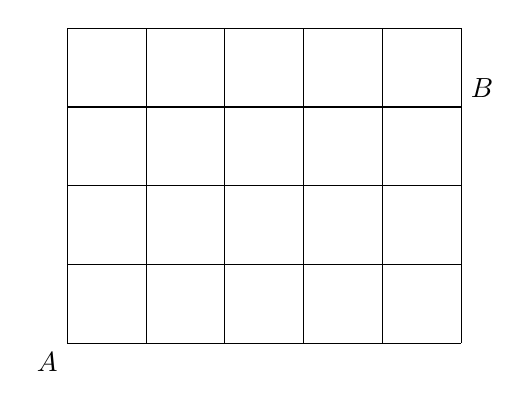
\begin{tikzpicture}
    \draw (0,0) grid (5,4);
    \draw (0,0) node[anchor=north east] {$A$};
    \draw (5,3) node[anchor=south west] {$B$};
    \end{tikzpicture}
    \caption{\label{fig:esercizio_21}Esercizio \ref{esercizio_21}}
    \end{figure}
    \item \label{esercizio_22} (1.22) Nel problema \ref{esercizio_21}, quanti sono i percorsi possibili che passano dal punto cerchiato in figura \ref{fig:esercizio_22}?
    \begin{figure}[ht]
    \centering
    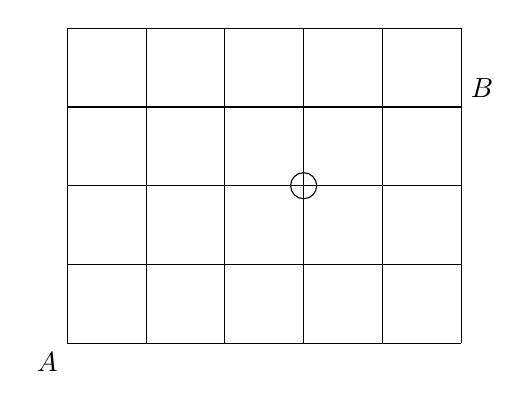
\begin{tikzpicture}
    \draw (0,0) grid (5,4);
    \draw (3,2) node[circle, draw] {};
    \draw (0,0) node[anchor=north east] {$A$};
    \draw (5,3) node[anchor=south west] {$B$};
    \end{tikzpicture}
    \caption{\label{fig:esercizio_22}Esercizio \ref{esercizio_22}}
    \end{figure}
    \item (1.23) Un laboratorio di psicologia che conduce degli esperimenti sui sogni dispone di 3 stanze con 2 letti ciascuna. In quanti modi si possono assegnare i letti a 3 coppie di gemelli in modo tale che ogni coppia di gemelli dorma nella stessa stanza?
    \item (1.27) In quanti modi si possono suddividere 12 persone in comitati di rispettivamente 3, 4 e 5 persone?
\end{enumerate}

\section{8 ottobre 2014}

\begin{enumerate}
    \item (1.13) Si consideri un gruppo di 20 persone. Quante sono le strette di mano se ciascuno d\`a la mano a tutti gli altri? $\sum_{k=1}^{n-1} k$. Equivale a chiedere: un grafo completo con $n$ vertici, quanti lati ha? Alternativamente, posso pensare una stretta di mano come un sottoinsieme di cardinalit\`a due dell'insieme delle persone, quindi il numero di strette di mano equivale al numero di sottoinsiemi di due elementi: $\binom{20}{2}$. Quindi vale anche $\sum_{k=1}^{n-1} k = \frac{n \cdot (n-1)}{2} = \binom{n}{2}$.
    \item (1.14) Quante sono le mani di cinque carte da poker? 32, 36 o 40 scelgo 5, a seconda se ci sono 4, 5 o 6 giocatori.
    \item (1.24) Sviluppare $\left( 3x^2 + y \right)^5$.
        \begin{align*}
        \left( 3x^2 + y \right)^5 = \\
        \binom{5}{0} \left( 3x^2 \right)^5 +
        \binom{5}{1} \left( 3x^2 \right)^4 y +
        \binom{5}{2} \left( 3x^2 \right)^3 y^2 + \\
        \binom{5}{3} \left( 3x^2 \right)^2 y^3 +
        \binom{5}{4} 3x^2 y^4 +
        \binom{5}{5} y^5 = \\
        243 \ x^{10} +
        5 \cdot 81 \ x^8 y +
        10 \cdot 27 \ x^6 y^2 +
        10 \cdot 9 \ x^4 y^3 +
        5 \cdot 3 \ x^2 y^4 +
        y^5 = \\
        243 \ x^{10} +
        405 \ x^8 y +
        270 \ x^6 y^2 +
        90 \ x^4 y^3 +
        15 \ x^2 y^4 +
        y^5
        \end{align*}
        $\binom{5}{2} = \binom{5}{3} = \binom{4}{2} + \binom{4}{1} = \binom{3}{2} + \binom{3}{1} + \binom{4}{1} = \binom{4}{1} + \binom{3}{1} + \binom{2}{2} + \binom{2}{1} = 4 + 3 + 2 + 1 = 10 $
    \item (1.25) Nel gioco del bridge ci sono 4 giocatori, a ciascuno dei quali sono distribuite 13 carte. Quante sono le possibili distribuzioni? $\binom{52}{13,13,13,13}$
\end{enumerate}

\section{10 ottobre 2014}

\begin{enumerate}
    \item Estraggo 3 carte da un mazzo di 40 (4 semi, 10 valori). Lo spazio campionario ha cardinalit\`a $\binom{40}{3}$ (tutti i sottoinsiemi di tre elementi di un insieme di 40 elementi), ossia 9880. Per simmetria gli esiti sono equiprobabili.
    \begin{enumerate}
        \item Calcolare la probabilit\`a di estrarre tutti assi. L'evento ha cardinalit\`a $\binom{4}{3} = 4 \Rightarrow $ la probabilit\`a dell'evento $P(E) = \frac{|E|}{|S|} \simeq 0{,}0004$.
        \item Calcolare la probabilit\`a che le tre carte abbiano lo stesso valore. Posso scegliere la prima carta in 40 modi, la seconda comunque ho scelto la prima in 3 modi (dovendo avere lo stesso valore), la terza in 2 modi. I possibili ordinamenti di questi tre elementi sono $3! = 6$. Ho quindi $\frac{240}{6} = 40$ possibili insiemi di tre carte uguali. La probabilit\`a dell'evento \`e $\frac{40}{9880} \simeq 0{,}004$.
        \item Calcolare la probabilit\`a che siano di tre valori differenti. Posso scegliere la prima carta in 40 modi. Per la seconda posso scegliere fra 9 valori con 4 semi, per la terza posso scegliere fra 8 valori con 4 semi. I possibili ordinamenti di questi tre elementi sono $3! = 6$. Ho quindi $\frac{40 \times 36 \times 32}{6} = 7680$ possibili insiemi di tre carte uguali. La probabilit\`a dell'evento \`e $\frac{7680}{9880} \simeq 0{,}777$.
    \end{enumerate}
    \item Lancio 2 dadi.
    \begin{enumerate}
        \item Calcolare la probabilit\`a che il risultato del primo lancio sia maggiore del secondo. La cardinalit\`a dell'evento \`e 15. La probabilit\`a \`e $\frac{15}{36} \simeq 0{,}41$.
    \end{enumerate}
\end{enumerate}

\section{13 ottobre 2014}

\begin{enumerate}
    \item (2.10) Il 60 per cento degli studenti di una scuola non indossano n\'e un anello n\'e una collana. Il 20 per cento porta un anello e il 30 per cento una collana. Se scegliamo uno studente a caso, qual \`e la probabilit\`a che indossi:
    \begin{enumerate}
        \item un anello o una collana? $P(A \cup C) = 1 - P((A \cup C)^{\mathsf{c}}) = 1 - 0{,}6 = 0{,}4$
        \item un anello e una collana? $P(A \cup C) = P(A) + P(C) - P(A \cap C) \Rightarrow P(A \cap C) = P(A) + P(C) - P(A \cup C) = 0{,}2 + 0{,}3 - 0{,}4 = 0{,}1$
    \end{enumerate}
    \item (2.12) Una scuola elementare offre corsi di tre lingue: uno dispagnolo, uno di francese e uno di tedesco. Ognuna di queste classi \`e aperta a ognuno dei 100 studenti della scuola. Nella classe di spagnolo ci sono 28 studenti, 26 in quella di francese e 16 in quella di tedesco. 12 studenti frequentano sia il corso di spagnolo che di francese, 4 sia quello di spagnolo che quello di tedesco e 6 sia quello di francese che di tedesco. Inoltre ci sono due studenti che frequentano tutti e tre i corsi di lingua.
    \begin{enumerate}
        \item Se scegliamo uno studente a caso, qual \`e la probabilit\`a che non segua alcun corso di lingua? $P(S^{\mathsf{c}} \cap F^{\mathsf{c}} \cap T^{\mathsf{c}}) = P((S \cup F \cup T)^{\mathsf{c}}) = 1 - P(S \cup F \cup T)$. Usiamo quindi il principio di inclusione ed esclusione per trovare $P(S \cup F \cup T) = P(S) + P(F) + P(T) - P(SF) - P(ST) -P(FT) + P(SFT) = \frac{28}{100} + \frac{26}{100} + \frac{16}{100} - \frac{12}{100} - \frac{4}{100} - \frac{6}{100} + \frac{2}{100} = \frac{1}{2}$.
        \item Se scegliamo uno studente a caso, qual \`e la probabilit\`a che frequenti un solo corso di lingua?
        \item Se scegliamo a caso 2 studenti, qual \`e la probabilit\`a che almeno 1 segua un corso di lingua?
    \end{enumerate}
    \item (2.15) Se supponiamo che tutte le $\binom{52}{5}$ mani di poker siano equiprobabili, qual \`e la probabilit\`a che venga servito:
    \begin{enumerate}
        \item un colore? (Una mano si definisce un colore se tutte e 5 le carte hanno lo stesso seme) Le possibili combinazioni di colore sono $4 \times \binom{13}{5}$.
        \item una coppia? (Questo capiter\`a quando le carte saranno $a, a, b, c, d$ con $a, b, c,$ e $d$ con valori distinti tra loro) Le possibili coppie sono $\frac{52 \times 48 \times 44 \times 40 \times 3}{5!}$, ossia il numero di modi in cui posso scegliere 4 carte con valori distinti per il numero di modi in cui posso scegliere la quinta carta in modo che abbia lo stesso valore della prima.
        \item una doppia coppia? (Questo capiter\`a quando le carte saranno $a, a, b, b, c$ con $a, b,$ e $c$ con valori distinti tra loro) Le possibili doppie coppie sono $\frac{52 \times 48 \times 44 \times 3^2}{5!} $, ossia il numero di modi in cui posso scegliere 3 carte con valori distinti per il numero di modi in cui posso scegliere la quarta e la quinta carta in modo che siano uguali rispettivamente alla prima ed alla seconda.
        \item un tris? (Questo capiter\`a quando le carte saranno $a, a, a, b, c$ con $a, b$ e $c$ con valori distinti tra loro)  I possibili tris sono $\frac{52 \times 48 \times 44 \times 6}{5!}$, ossia il numero di modi in cui posso scegliere 3 carte con valori distinti per il numero di modi in cui posso scegliere la quarta e la quinta carta in modo che siano uguali alla prima.
        \item un poker? (Questo capiter\`a quando le carte saranno $a, a, a, a, b$ con $a$ e $b$ con valori distinti tra loro) I possibili poker sono $\frac{52 \times 48 \times 6}{5!}$, ossia il numero di modi in cui posso scegliere 2 carte con valori distinti per il numero di modi in cui posso scegliere la terza, la quarta e la quinta carta in modo che siano uguali  alla prima.
    \end{enumerate}
\end{enumerate}

\section{15 ottobre 2014}

\begin{enumerate}
    \item (2.17) Se 8 torri vengono disposte a caso su di una scacchiera, si calcoli la probabilit\`a che nessuna torre possa mangiarne un'altra. Cio\`e, si calcoli la probabilit\`a che nessuna riga n\'e colonna contenga pi\`u di una torre.
    \item (2.18) Scegliamo due carte a caso da un mazzo di 52 carte da gioco. Qual \`e la probabilit\`a che formino un blackjack? Cio\`e, qual \`e la probabilit\`a che una delle due carte sia un asso e l'altra sia un dieci, un fante, una donna o un re?
    \item (2.19) Due dadi equilibrati hanno entrambi due facce di colore rosso, due nere, una gialla e una bianca. Se lanciamo i due dadi, qual \`e la probabilit\`a che si ottenga in entrambi i dadi una faccia del medesimo colore?
\end{enumerate}

\section{17 ottobre 2014}

\begin{enumerate}
    \item (2.27) Un'urna contiene 3 palline rosse e 7 nere. Due giocatori, A e B, estraggono uno alla volta una pallina dall'urna fino a che non viene estratta la prima pallina rossa. Si determini la probabilit\`a che A estragga la pallina rossa. (A estrae la prima pallina, B la seconda, A la terza e cos\`i via. Le estrazioni vengono fatte senza reinserimento.)
    \item (2.28) Un'urna contiene 5 palline rosse, 6 blu e 8 verdi. Se estraiamo un blocco di 3 palline, qual \`e la probabilit\`a che le palline abbiano
    \begin{enumerate}
        \item il medesimo colore;
        \item tre colori differenti?
    \end{enumerate}
    Si ripeta l'esercizio sotto l'ipotesi che estraiamo le tre palline una alla volta e che dopo ogni estrazione, segnamo che colore \`e uscito e reinseriamo la pallina nell'urna prima del'estrazione successiva. Questo procedimento \`e noto come campionamento con reinserimento.
    \item (2.31) Una squadra di basket \`e formata da 3 giocatori (una guardia, un'ala e un centro).
    \begin{enumerate}
        \item Se scegliamo un giocatore a caso da tre quadre formate nel modo precedente, qual \`e la probabilit\`a che venga selezioanta una nuova squadra con guardia, ala e centro?
        \item Qual \`e la probabilit\`a che i 3 giocatori selezionati giochino tutti e tre nel medesimo ruolo?
    \end{enumerate}
    \item (2.33) Una foresta contiene 20 alci, dei quali 5 vengono catturati, marchiati e quindi liberati. Dopo un certo tempo 4 delle 20 alci vengono catturate. Qual \`e la probabilit\`a che 2 di esse siano marchiate? Che ipotesi state facendo?
    \item (2.35) A un congresso partecipano 30 fisici e 24 matematici. Tre dei 54 partecipanti al congresso vengono scelti a caso per comporre un gruppo di lavoro. Qual \`e la probabilit\`a che almeno un matematico ne faccia parte?
    \item (2.37) Una professoressa assegna agli studenti 10 problemi, informandoli che l'esame finale consister\`a in 5 di questi scelti a caso. Se uno studente \`e riuscito a risolverne 7, qual \`e la probabilit\`a che risponda esattamente a
    \begin{enumerate}
        \item 5 dei problemi dell'esame finale;
        \item almeno 4 dei problemi dell'esame finale?
    \end{enumerate}
    \item (2.39) In una citt\`a ci sono 5 alberghi. Se un giorno 3 persone scelgono a caso un albergo dove pernottare, qual \`e la probabilit\`a che ognuno scenda in un albergo diverso? Che ipotesi state facendo?
\end{enumerate}

\section{27 ottobre 2014}

\begin{enumerate}
    \item (2.44)
    \item (2.45)
    \item (2.47)
    \item (2.48)
    \item (3.1)
    \item (3.6)
\end{enumerate}

Lancio 2 dadi. E = ``almeno uno dei due d\`a 6'', F = ``i dadi danno numeri diversi''. Calcolare P(E|F).

Lo spazio campionario $S = \{(a, b) : a, b \in \{1 \dots 6\}\}$ ha esiti equiprobabili, quindi:
\[
P(E | F) = \frac{|E \cap F|}{|F|}
\]
$|F| = 6 \cdot 5 = 30$. Bisogna sapere $|E \cap F|$.

% disegnare il quadratone di lato sei e togliere la diagonale.

\section{31 ottobre 2014}

\begin{enumerate}
    \item (2.20) $P(E^{c} \cap F^{c}) = P((E \cup F)^{c}) = 1 - P(E \cup F) = 1 - P(F) - P(E) + P(E \cap F)$

    La probabilit\`a che io abbia un black jack \`e uguale a quella che il banco abbia un black jack.
    \item (3.10)
    \item (3.11)
    \item (3.12)
\end{enumerate}

\section{3 novembre 2014}

\begin{enumerate}
    \item (3.14)
    \item (3.15)
    \item (3.16)
    \item (3.43)
\end{enumerate}

\section{5 novembre 2014}

\begin{enumerate}
    \item (3.23)
    \item (3.31)
    \item (3.47)
\end{enumerate}

\section{7 novembre 2014}

\begin{enumerate}
    \item (3.9)
    \item (3.20)
    \item (3.48)
    \item (3.66)
\end{enumerate}

\section{14 novembre 2014}

\begin{itemize}
    \item (3.64)
    \item (4.1)
    \item (4.2)
    \item (4.4)
\end{itemize}

\section{17 novembre 2014}

\begin{itemize}
    \item (3.73)
    \item (4.13)
    \item (4.14)
\end{itemize}


\section{19 novembre 2014}

\begin{itemize}
    \item (4.21)
    \item (4.23)
\end{itemize}

\section{21 novembre 2014}

\begin{itemize}
    \item (4.35)
    \item (4.38)
    \item (4.41)
    \item (4.48)
\end{itemize}

\section{24 novembre 2014}

\begin{itemize}
    \item (4.40)
    \item (4.43)
\end{itemize}


\section{28 novembre 2014}

\begin{itemize}
    \item (4.49)
    \item (4.51)
    \item (4.52)
    \item (4.53)
\end{itemize}

\section{1 dicembre 2014}

\begin{itemize}
    \item (4.75)
    \item (4.79)
\end{itemize}




\section{3 dicembre 2014}

\begin{itemize}
    \item (4.81)
    \item (6.1)
\end{itemize}

\section{10 dicembre 2014}

\begin{itemize}
    \item (7.6)
    \item (7.7)
    \item (7.13)
    \item (7.30)
    \item (7.36)
    \item (7.37)
    \item (7.41)
\end{itemize}

\end{document}
